\documentclass[
  % More capable input encoding than latin-1.
  utf8,
  %
  % For vertical whitespace between paragraphs.  This comes down to more
  % than just using parskip.sty, so it's better to use this class option.
  parskip,
  %
  % If you intend to really use margin paragraphs (not recommended!).
  % S5MP,
  %
  % Produce output with crop marks and paper size A4.  Liu-Tryck should like this.
  % Automatically adds information, including the physical page number, at the top of each page.
  % Add option 'noInfo' to suppress the info at the top of each page when using option 'crop'.
  % crop,
  %
  % Font options: 'kp' (default), 'times', 'lm'.
  % The KpFonts (loaded using 'kp'), is the most complete font among the provided options.
  % Among other, it supports slanted small caps.  See rtthesis.cls for more details regarding the font options.
  times,
  %
  % Good options to KpFonts. XXX use kpfonts?
  %largesmallcaps,intlimits,widermath,
  %
  % See comments in the results chapter of this document for more information on these options!
  sharecounter,nobreak,definition=marks,
  %
  % If you want to cite references by numbers, use this option.
  numbers,
  %
  % Use option 'noparts' if you do not make use of part divisions.
  noparts
]{rtthesis/rtthesis}
\usepackage{mythesis}


\begin{document}
\selectlanguage{english}
\makeFrontPage
\frontmatter
\maketitle
\makeLibraryPage{%\textit{Short and concise describe the problem at hand with results and conclusions.}

%\textit{Normally max 150 words, no references or line breaks. Heh.}

%\textit{This sucks}

%A recommender system based on \textit{katz-eig} and \textit{link-analysis} with analysis and tuning of the learning parameters is designed. The parameter $\beta$ is fixed for \textit{katz-eig} and the parameter $K$ is found using hill climbing. $\eta$ is locked to $\eta = 1 \text{ or } -1$ for \textit{link-analysis} and $\gamma$ is found using adaptive hill climbing.

1. Why

2. How

3. (Some results...)

4 Conclusions

SELL the thesis!!!

Implicit feedback recommender systems are important for Comordo Technologies.... Make recommendations for users without them having to do anything.
}

\begin{abstract}[english]
  %\textit{Short and concise describe the problem at hand with results and conclusions.}

%\textit{Normally max 150 words, no references or line breaks. Heh.}

%\textit{This sucks}

%A recommender system based on \textit{katz-eig} and \textit{link-analysis} with analysis and tuning of the learning parameters is designed. The parameter $\beta$ is fixed for \textit{katz-eig} and the parameter $K$ is found using hill climbing. $\eta$ is locked to $\eta = 1 \text{ or } -1$ for \textit{link-analysis} and $\gamma$ is found using adaptive hill climbing.

1. Why

2. How

3. (Some results...)

4 Conclusions

SELL the thesis!!!

Implicit feedback recommender systems are important for Comordo Technologies.... Make recommendations for users without them having to do anything.

\end{abstract}
\begin{acknowledgments}
  All thanks to Veronica who has been a pillar and a saint during these laborous times.

  \addvspace{1em}
  \begin{flushright}
    \textit{%
      Linköping, Januari 2015\\
      Jonas Hietala%
    }
  \end{flushright}
\end{acknowledgments}

\tableofcontents
%\include{notation}

\mainmatter

\chapter{Introduction}\label{cha:intro}

The introduction chapter presents the purpose and the goals of the thesis, what questions the thesis aims to answer, the limitations of the thesis and the contributions of this thesis. An outline of the thesis concludes the chapter.


\section{Introduction}\label{sec:intro:intro}

The introduction chapter presents the purpose and the goals of the thesis, what questions the thesis aims to answer and the limitations of the thesis.

This thesis examines the construction of a recommender system and the evaluation of two different recommender algorithms, \textit{link-analysis} and \textit{katz-eig}. Both of the algorithms had their parameter space analysed and different optimization strategies were evaluated using several different datasets. The recommender system was built for Comordo Technologies as their recommender system to later be built upon and extended.

\textit{Conclusion/result summary here}

\Warning[TODO]{ A short summary of the conclusions/results here? }



\section{Problem definition}\label{sec:intro:problem}

The purpose of this thesis can be split in two larger parts. The first is to lay the foundation of Comordo Technologies' recommender system which could later be built upon and extended. At the end of this thesis the goal is to have a recommendation system which could load data supplied by Comordo's clients, produce recommendations and store them together with their recommendations in a database.

The second part is to analyze and create optimization strategies for \textit{katz-eig} and \textit{link-analysis} which optimize the algorithm's parameters for different datasets automatically. Parameter optimization should be done in a reasonable amount of time so the system can be commercially useful.

The recommendation algorithms depend on a couple of parameters which directly affects the quality of the recommendations made and the parameter values are different depending on the dataset the recommendations are being made for.  Recommendation quality, or how good the recommendations are, is measured by the probability that a user interacts with the recommendation given by the system in the future where only recommendations to items not previously interacted with can be given. The goal of the optimization process is to maximize this probability for a specific dataset.

Core parts of the recommendation algorithms \textit{katz-eig} and \textit{link-analysis} existed before the thesis, but they were only runnable as Matlab scripts without any data handling and they lacked parameter tuning. There were also some optimization issues with the implementations. Focus is not on porting them to a different language or platform, which could improve them speed wise, but to adapt the existing code.

\newpage
\subsection{Guiding questions}\label{sec:intro:questions}

\begin{itemize}

    \item How can a recommender system be designed to allow for easily extendible input- and output handling?


    \item How can learning and recommendation using \textit{link-analysis} and \textit{katz-eig} be performed in practice, with regards to speed and recommendation quality?

        \begin{itemize}
            \item How shall learning and optimization of their parameters be done?
        \end{itemize}

        To answer that question, an exploration of the function space of the parameters with regards to the evaluation criteria might be necessary.

\end{itemize}



\section{Limitations}\label{sec:intro:limitations}

\textit{Avgränsningar?}

Although the goal is to handle real time data, the data handled will still be of a smaller size, as some of the algorithms are not very fast. The algorithms are not optimized enough to handle the larger data sets which limits the abilities to make optimizations for them.

The algorithm's perhaps slow runtime will be a consideration during the selection and evaluation of optimization techniques.

There are different kinds of interaction history such as ratings, interaction count and like or dislike. We will only consider a simple kind of interaction history where each user-product pair will be a binary value, no matter how many times the user has interacted with the product. This is to simplify the analysis, different types of interaction history benefits from different types of algorithms and evaluations.

The existing algorithms are currently written in Matlab which might negatively impact the runtime and handling of larger datasets. Focus will not be on porting them to a different language, which could improve them speed wise, but focus will be on optimization the Matlab code.



\section{Contributions}\label{sec:intro:contributions}

A first version of Comordo's recommender system is built based around the recommender algorithms \textit{katz-eig} and \textit{link-analysis} with parameter optimization and flexible input- and output handling. The designed system can later be built upon and extended.

The parameter space over \textit{F-measure} for \textit{katz-eig} and \textit{link-analysis} is analyzed and for these datasets changes in $\beta$ for \textit{katz-eig}  have negligible effect. There are two plateaus at $\eta < 0$ and $\eta > 0$ for \textit{link-analysis} and either one can give a global maximum.

An effective parameter optimization strategy for \textit{katz-eig} is to fix $\beta = \| A_{train} \|_2$ and optimize $K$ using a hill climbing algorithm. For \textit{link-analysis} an effective strategy is to set $\eta = 1$ or $\eta = -1$ and optimize $\gamma$ using an adaptive hill climbing algorithm.



\section{Outline of the report}\label{sec:intro:outline}

This thesis consists of two parts. A system development part where a first version of Comordo's recommender system is built. The second part consists of an analysis of the parameter space and optimization strategies for the algorithms' parameters. The system development part is concentrated to chapter 4 and the parameter analysis to chapter 6.

\begin{description}
    \item[Chapter 2] introduces the mathematical background for the thesis. The recommendation model and the learning process along with the recommendation algorithms \textit{katz-eig} and \textit{link-analysis} are presented.
    \item[Chapter 3] discusses work related to this thesis.
    \item[Chapter 4] covers the system development part of this thesis. Beginning with the given system development task and then presenting the constructed recommender system.
    \item[Chapter 5] presents the datasets used by this thesis. Contains an analysis of the datasets with respect to interactions and clusters.
    \item[Chapter 6] covers the parameter analysis and optimization. The chapter begins with an analysis of the algorithms and the parameter space and finishes with a comparison of different optimization techniques and a comparison between the algorithms.
    \item[Chapter 7] contains a discussion about the thesis and presents ideas for future work. Recommender systems in general and the one built are discussed. Then discussion about the datasets, the evaluation method and finally parameter tuning follow.
    \item[Chapter 8] concludes with the conclusions of this thesis.
    \item[Appendix A] lists the optimized parameters for each dataset and algorithm.
    \item[Appendix B] presents the available source code. Only an example reader plugin is available.
    \item[Appendix C] describes the test setup used by this thesis.
\end{description}





\chapter{Background}\label{cha:background}
\vspace{-0.5cm} % Just making things pretty, harr!!!!!

This chapter describes the background of the thesis and the task given by given by Comordo for the construction of the recommender system which is the main purpose of the thesis from Comordo's point of view. Then a rundown of mathematical theory of the used recommendation model and description of the used algorithms follow.

%Then background theory about supervised learning, the used recommendation model and evaluating recommendations and a summary of optimization strategies are given.  Descriptions of the algorithms \textit{katz-eig} and \textit{link-analysis} follow.

Comordo Technologies is a startup in recommendation systems driven inside the bounds of LiU's incubator LEAD in Linköping and will in the future offer a cloud service for e-commerce. The base for the recommendation system is algorithms based on predication and machine learning. At the start of this thesis the company stood to build a first version of it's recommendation system.

Comordo focuses on generating personal recommendations using \textit{implicit feedback} aimed at e-commerce using purchase history for users as their main focus. The end product aims to be a remote API where e-commerce clients queries for precomputed recommendations made for their users.


\section{Use case}\label{sec:use}

\begin{enumerate}
    \item Purchase history and product data is provided by e-commerce clients and consumed by the recommender system.
    \item Load algorithms with purchase history and is run on a nightly basis.
    \item Repopulate recommendation database with new recommendations.
    \item Final customers visit the e-commerce website and are given recommendations delivered to the website via Commordo's remote API.
\end{enumerate}


\section{System overview}\label{sec:sysoverview}

Figure \ref{fig:sysoverview} is a sketch of Commordo's recommender system, as planned for at the start of the thesis.

\begin{figure}[h!]
  \centering
    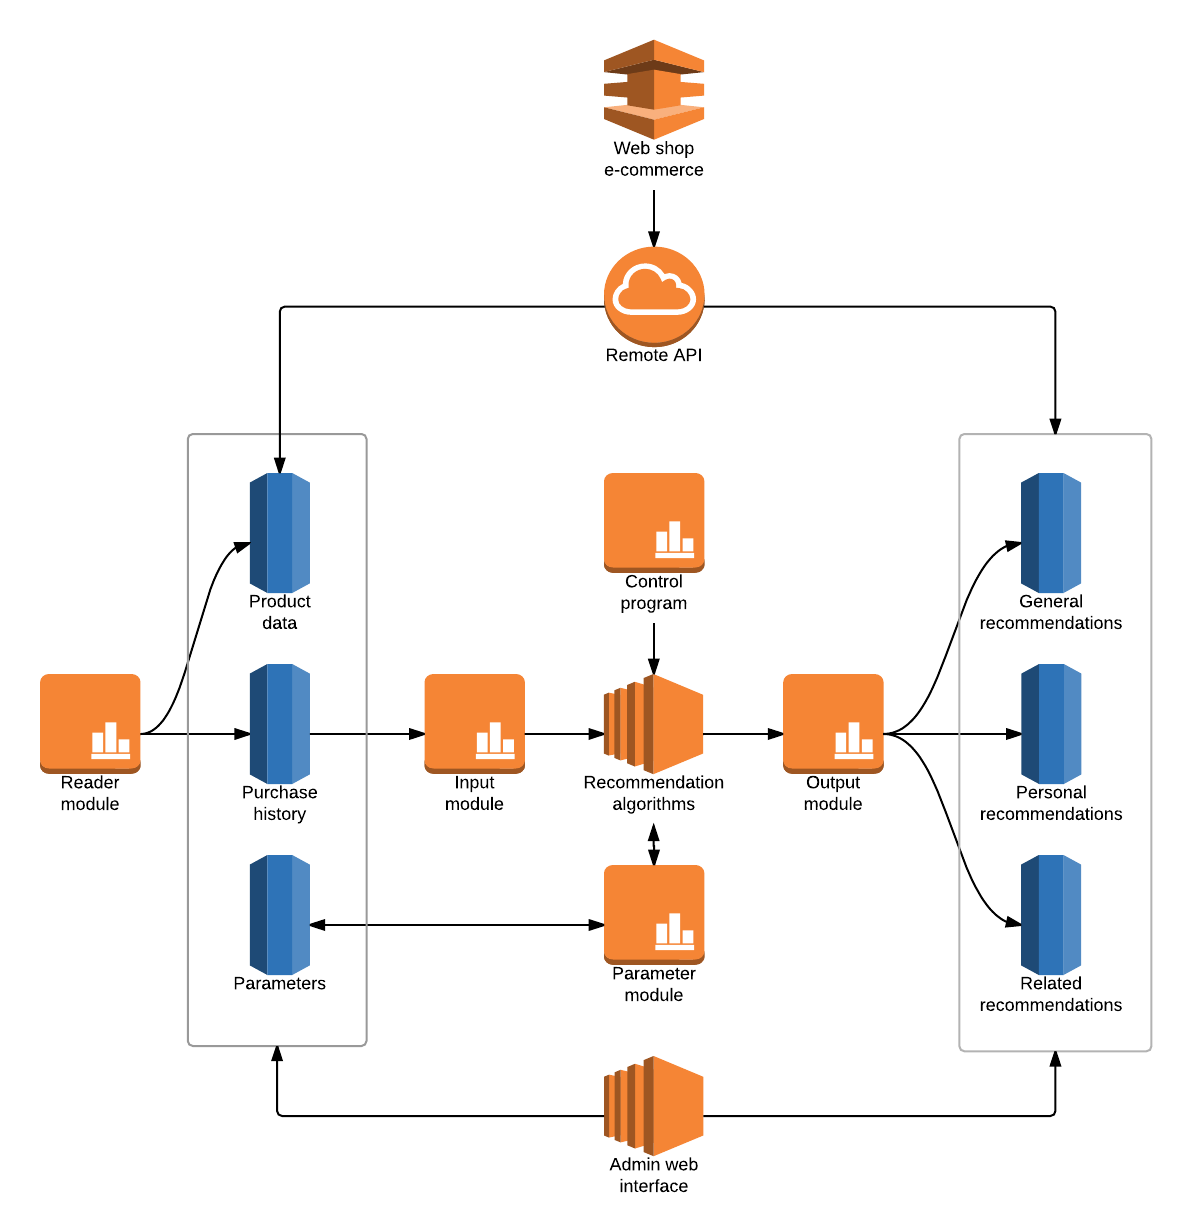
\includegraphics[width=0.9\textwidth]{fig/system_overview.png}
  \caption{Commordo's system sketch}
  \label{fig:sysoverview}
\end{figure}

\FloatBarrier

\begin{description}
    \item[Reader module] is responsible for reading data files provided by Commordo's clients.
    \item[Input module] provides the algorithms with transformed data.
    \item[Output module] populates the database with recommendations.
    \item[Control program] handles learning and optimization of the algorithms.
    \item[Parameter module] stores and adjusts parameters the algorithms use.
    \item[Remote API] is a REST based API, the endpoint for Commordo's clients.
    \item[Admin web interface] is a user friendly way for e-commerce clients to customize system settings and view recommendations.
\end{description}



\section{Task}\label{sec:task}

The task for this thesis was to complete the backend of Commordo's system. This includeded the reader, input, output and parameter modules, the storage of purchase history and parameters and algorithms for parameter tuning. The other databases were be provided, but with some level of adaptation. The recommender algorithms were given. The admin interface and the remote API are not included in this thesis.


\chapter{Theory}\label{cha:theory}


\subsection{Model}\label{sec:background:theory:model}

Given a set of users $U$, a set of items $I$ and an interaction history $h_{u, i}$ given in \textit{unweighted binary form}

\begin{equation}\label{eq:hist}
    h_{u, i} = \begin{cases}
        1 \quad \text{if user $u$ has interacted with item $i$} \\
        0 \quad \text{otherwise}
    \end{cases}
\end{equation}

the \textit{recommender problem} is defined by producing a set of recommendations $r_{u, i}$

\begin{equation}\label{eq:binrec}
    r_{u, i} = \begin{cases}
        1 \quad \text{if item $i$ is recommended to user $u$} \\
        0 \quad \text{otherwise}
    \end{cases}
\end{equation}

to maximize the probability that user $u$ will want to interact with item $i$ in the future, for all users and items.  When $r_{u, i}$ is binary this is a \textit{binary classification} problem. This definition is applicable for \textit{implicit feedback} systems which passively track different sorts of user behaviour. For example link following, interaction time and purchase history.

The recommender problem can be extended to the \textit{Top-N recommender problem} by introducing constraints \eqref{eq:constrain_N} which states that only $N$ recommendations can be presented for each user.

\begin{equation}\label{eq:constrain_N}
    \sum_i r_{u, i} \leq N \quad \forall u
\end{equation}


A variation of the recommender problem is when the interaction history is in \textit{weighted form}, when the values increase with each interaction

\begin{equation}\label{eq:whist}
    h_{u, i} = \begin{cases}
        x \quad \text{user $u$ has interacted $x$ times with item $i$} \\
        0 \quad \text{otherwise}
    \end{cases}
\end{equation}

for example $h_{u, i} = 2$ means that the user $u$ has interacted with item $i$ 2 times. It is possible to allow \textit{implicit feedback} systems to log partial interactions, so $h_{u, i} = 0.7$ could mean that user $u$ has watched 70\% of the movie $i$, in the context of movie watching. \citep{hu2008collaborative}

The converse of \textit{implicit feedback} is \textit{explicit feedback} where the users give direct input regarding their preferences, for example with movie ratings or with likes and dislikes.  Here the definition of the interaction history $h_{u, i}$ is the users' rating history.

\begin{equation}
    h_{u, i} = \begin{cases}
        x \quad \text{the rating $x$ user $u$ gave item $i$} \\
        \emptyset \quad \text{if the user $u$ did not rate item $i$}
    \end{cases}
\end{equation}

\Warning[TODO]{ Uses h for all equations? }

With ratings $r_{u, i}$ changes to $r_{u, i} = \hat{x}$ where $\hat{x}$ is the rating user $u$ is predicted to give item $i$.

\section{The link-analysis algorithm}\label{sec:linkanalysis}

%\textit{Cleanup, mostly description from article. Reduce information?}

The \textit{link-analysis} algorithm, as presented by \cite{huang2004link} and further discussed in \cite{huang2007comparison}. See the articles for more information and in-depth examples. What follows is a condensed description of how the algorithm works.

The algorithm is an adaptation of HITS \cite{kleinberg1999authoritative} which is a web page ranking algorithm to the recommendation domain. The original algorithm distinguish between \textit{Authoritative} pages which definitely contain high-quality information and \textit{Hub} pages which are comprehensive lists of links to authoritative pages. \citep{huang2007comparison}

The adaptation to the recommendation domain is achieved by introducing the \textit{product representativeness} score $\PR$ and the \textit{consumer representativeness} score $\CR$.

The \textit{product representativeness} score $\PR(i, u)$ can be seen as a measure of the item $i$'s level of interest with respect to user $u$, or in other words $i$'s authority of $u$'s interests in $i$.

The \textit{consumer representativeness} score $\CR(u, \hat{u})$ measures how well $u$ as a hub for $\hat{u}$ associates with products of interests to $\hat{u}$.

If $h_{u, i}$ is the user-item interaction history as defined by \ref{eq:hist} and $h$ is the interaction matrix then a recursive definition of the authority and hub scores can be defined as

\begin{equation}
    \PR = h' * \CR
\end{equation}

\begin{equation}
    \CR = B * \PR + \CR_0
\end{equation}

Where $B$ is a matrix such that:

\begin{equation}
    B_{u, i} = \frac{ h_{u, i} }{ \left(\sum_{i} h_{u, i}\right)^\gamma }
\end{equation}

Meaning $B$ normalizes the representativeness score a costumer receives from linked products by dividing it with the total number of products the customer is linked to.  $\gamma$ controls the extent to which a consumer is penalized for making many purchases.

$\CR_0$ is defined as

\begin{equation}
    \CR_{i, j}^0 = \begin{cases}
        \eta \quad \text{if } \; i = j \\
        0    \quad \text{otherwise}
    \end{cases}
\end{equation}

in other words $\CR_0 = \eta * I_M$ where $I_M$ is an $M x M$ identity matrix and $M$ is the number of users.  It is included to maintain the high representativeness score for the target users themselves. This also necessitates a normalization step to keep the values on a consistent level.

In summary the \textit{link-analysis} algorithm follow these steps:

\begin{enumerate}
    \item Construct the interaction matrix $A$ and the associating matrix $B$.

    \item Set $\CR_0 = \eta * I_M$.
    \item At each iteration $t = 1, \ldots, t_{max}$ perform:

        \begin{enumerate}
            \item $\PR_t = h' * \CR_{t- 1}$
            \item $\CR_t = B * \PR_t$
            \item Normalize $\CR_t$ so each column adds up to 1
            \item $\CR_t = \CR_t + \CR_0$
        \end{enumerate}

        Repeat until convergence.

    \item Predicted user-item interaction is given by $\mathit{pval} = \PR'$.

\end{enumerate}

There are two parameters to the algorithm: $\gamma$ and $\eta$.
%\Warning[TODO]{ Describe them, what's their purpose }



\subsection{katz-eig}

There are two parameters to \textit{katz-eig}: $\beta$, the link diminishing factor and $K$ specifying the $K$-rank approximation. $\beta$ is a continous value satisfying $0 < \beta \leq \frac{1}{\|A_{train}\|_2}$. If $\beta = 0$ then the algorithm will only output 0 and if $\beta > \frac{1}{\|A_{train}\|_2}$ the iterations will not converge. $K > 0$ is a discrete value.

What follows is plots over both of the parameters $K$ and $\beta$. The plots are evaluated using \textit{F-measure} w.r.t. the test set using top-10 recommendations.

\begin{figure}[h!]
\centering
\begin{minipage}{.5\textwidth}
    \centering
    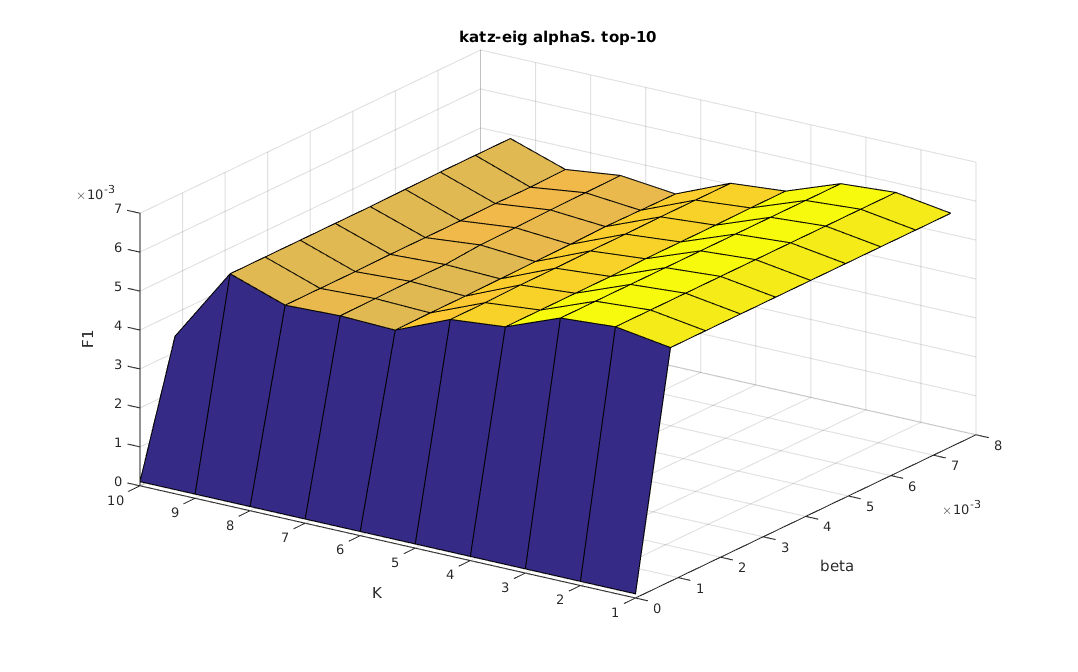
\includegraphics[width=\linewidth]{fig/katzeig_beta_k/alphaS_katzeig.png}
    \captionof{figure}{\textit{alphaS}}
\end{minipage}%
\begin{minipage}{.5\textwidth}
    \centering
    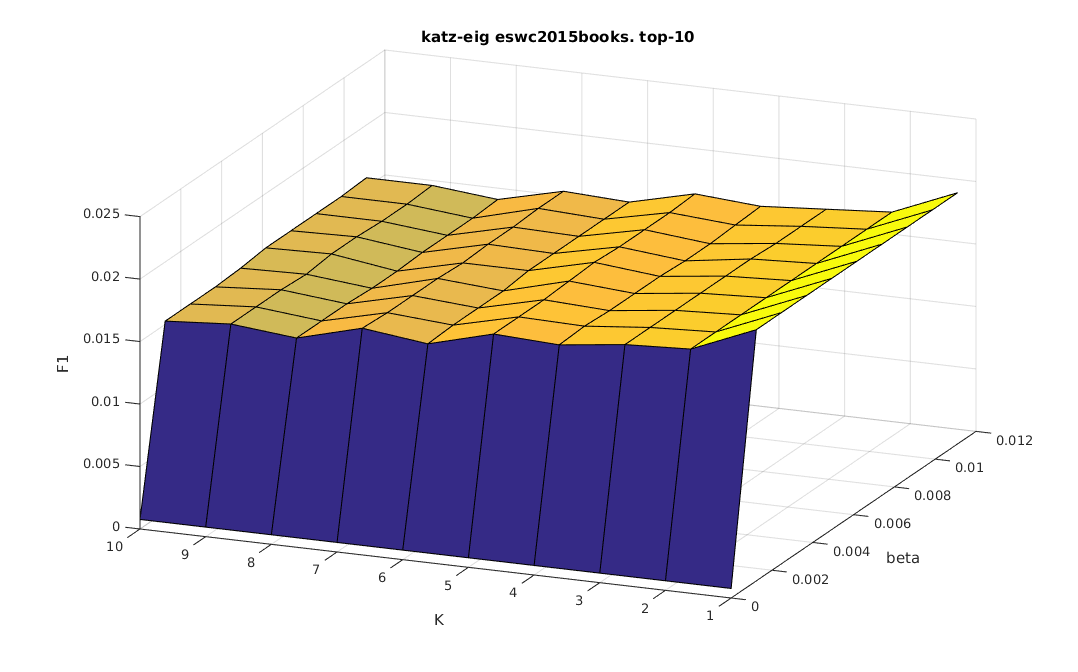
\includegraphics[width=\linewidth]{fig/katzeig_beta_k/eswc2015books_katzeig.png}
    \captionof{figure}{\textit{eswc2015books}}
\end{minipage}
\end{figure}

\begin{figure}[h!]
\centering
\begin{minipage}{.5\textwidth}
    \centering
    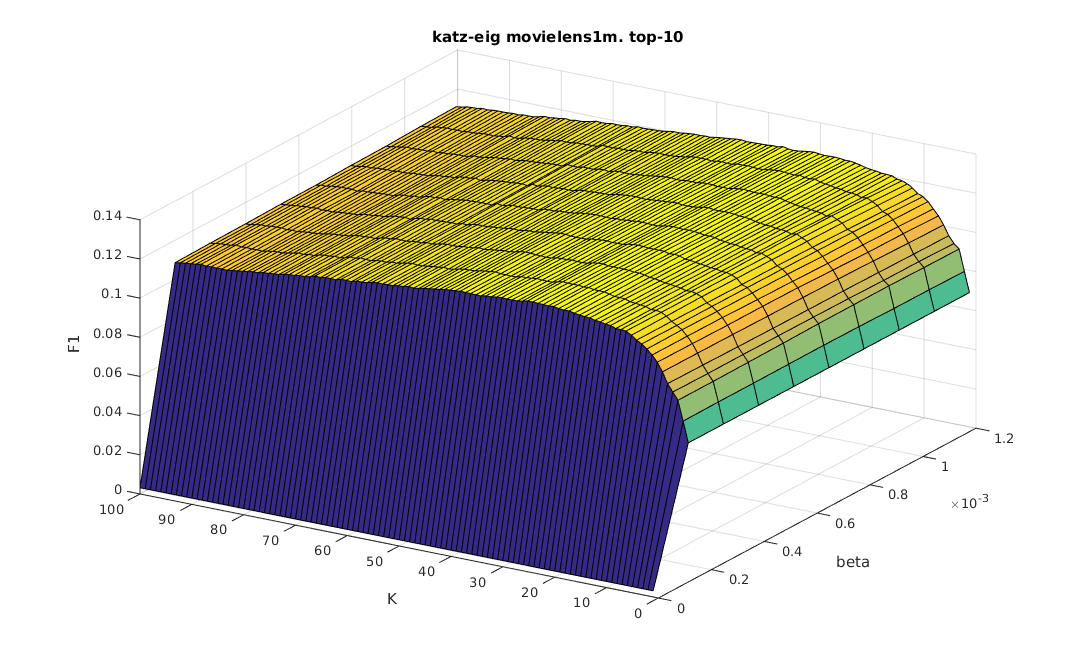
\includegraphics[width=\linewidth]{fig/katzeig_beta_k/movielens_katzeig.png}
    \captionof{figure}{\textit{movielens1m}}
\end{minipage}%
\begin{minipage}{.5\textwidth}
    \centering
    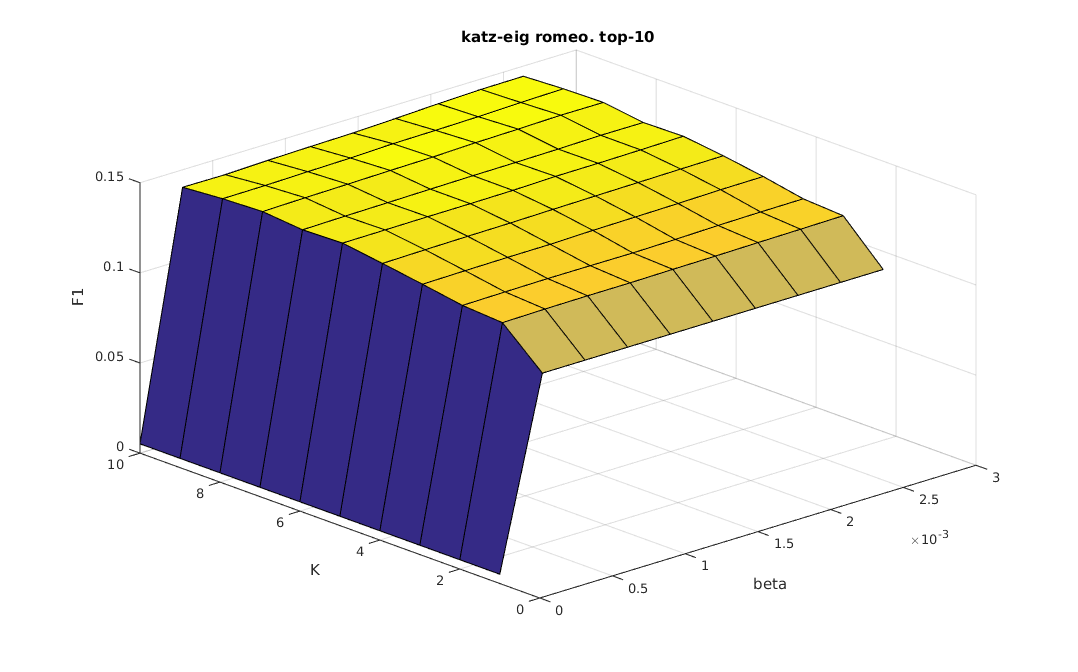
\includegraphics[width=\linewidth]{fig/katzeig_beta_k/romeo_katzeig.png}
    \captionof{figure}{\textit{romeo}}
\end{minipage}
\end{figure}




It seems like $beta$ doesn't have a very big impact on the function value. Some plots with a fixed $K$ follows to better see differences.

The range examined is $0 < \beta \leq \beta_{max} = \frac{1}{\|A_{train}\|_2}$ with a $K$ selected to fit the specific dataset. Again evaluated using \textit{Precision}, \textit{Recall} and \textit{F-measure} w.r.t. the test set using the top-10 recommendations.

\FloatBarrier

\begin{figure}[h!]
\centering
\begin{minipage}{.5\textwidth}
    \centering
    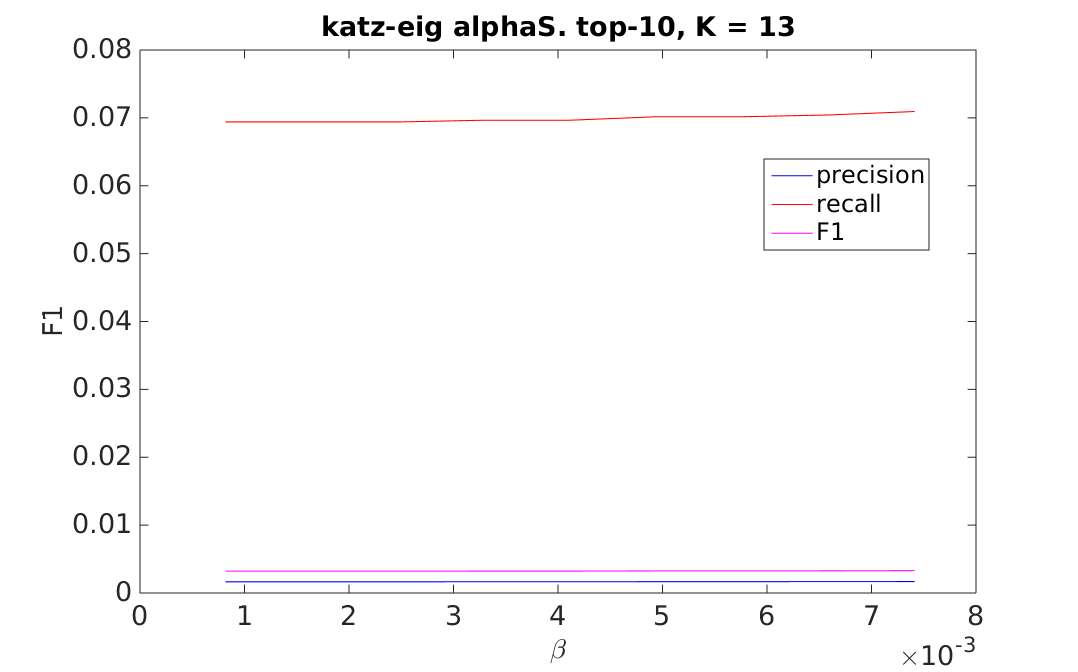
\includegraphics[width=\linewidth]{fig/katzeig_beta/alphaS_katzeig_beta.png}
    \captionof{figure}{\textit{alphaS}.
        $\beta_{max}$ is the best value with a $1.9\%$ diff between the minimum and the maximum \textit{F1} value.}
\end{minipage}%
\begin{minipage}{.5\textwidth}
    \centering
    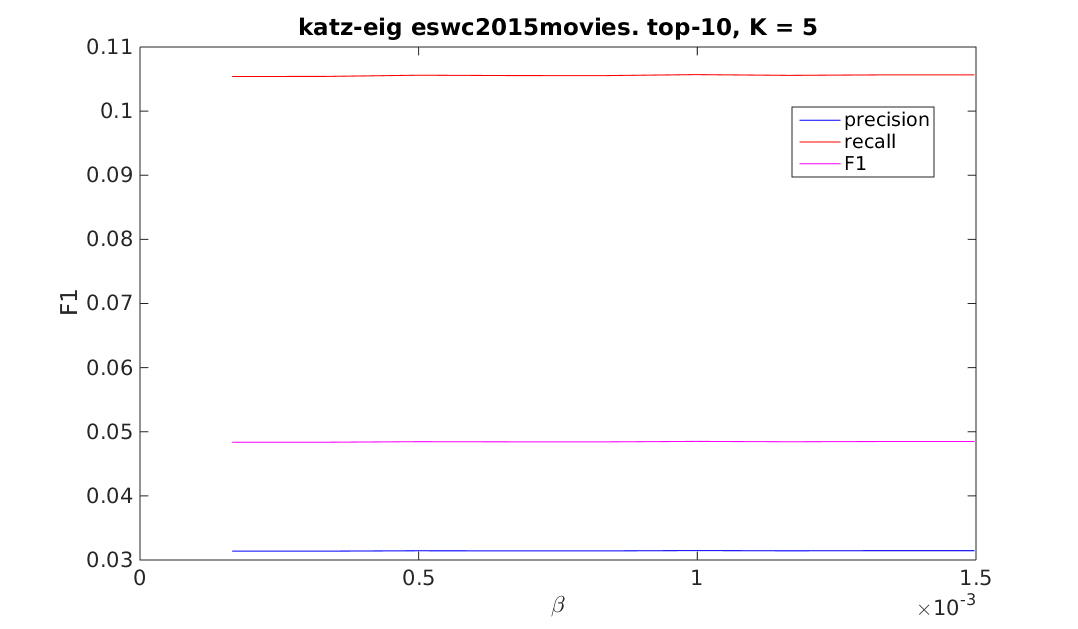
\includegraphics[width=\linewidth]{fig/katzeig_beta/eswc2015movies_katzeig_beta.png}
    \captionof{figure}{\textit{eswc2015movies}.
        $\beta_{max}$ is not the best value with a $0.3\%$ diff between the minimum and the maximum \textit{F1} value.}
\end{minipage}
\end{figure}

\begin{figure}[h!]
\centering
\begin{minipage}{.5\textwidth}
    \centering
    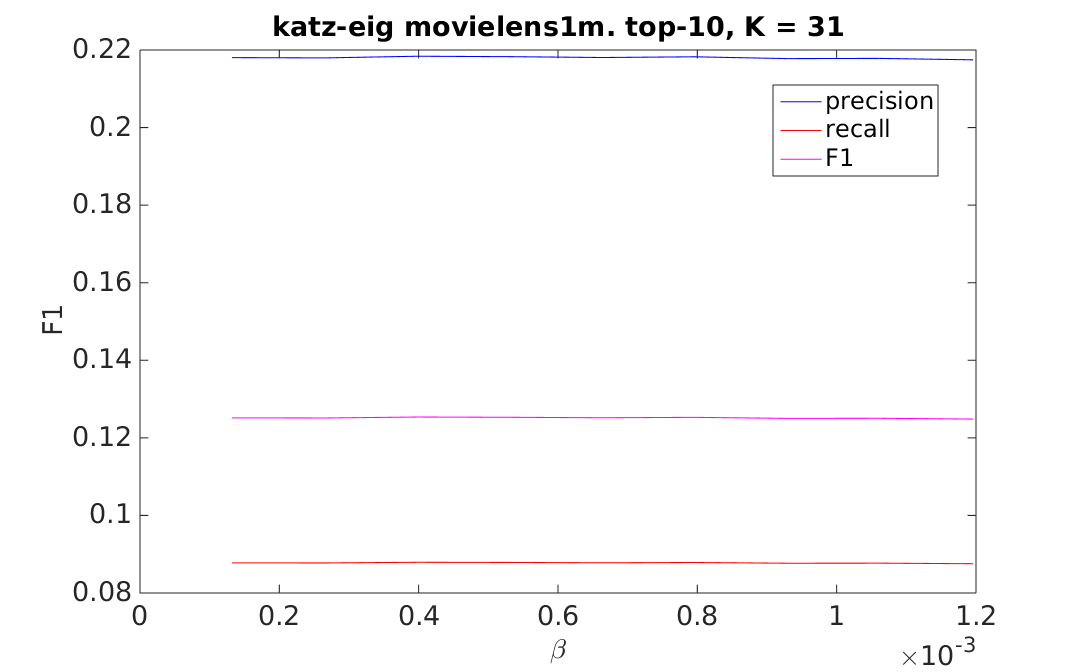
\includegraphics[width=\linewidth]{fig/katzeig_beta/movielens_katzeig_beta.png}
    \captionof{figure}{\textit{movielens1m}.
        $\beta_{max}$ is not the best value with a $0.41\%$ diff between the minimum and the maximum \textit{F1} value.}
\end{minipage}%
\begin{minipage}{.5\textwidth}
    \centering
    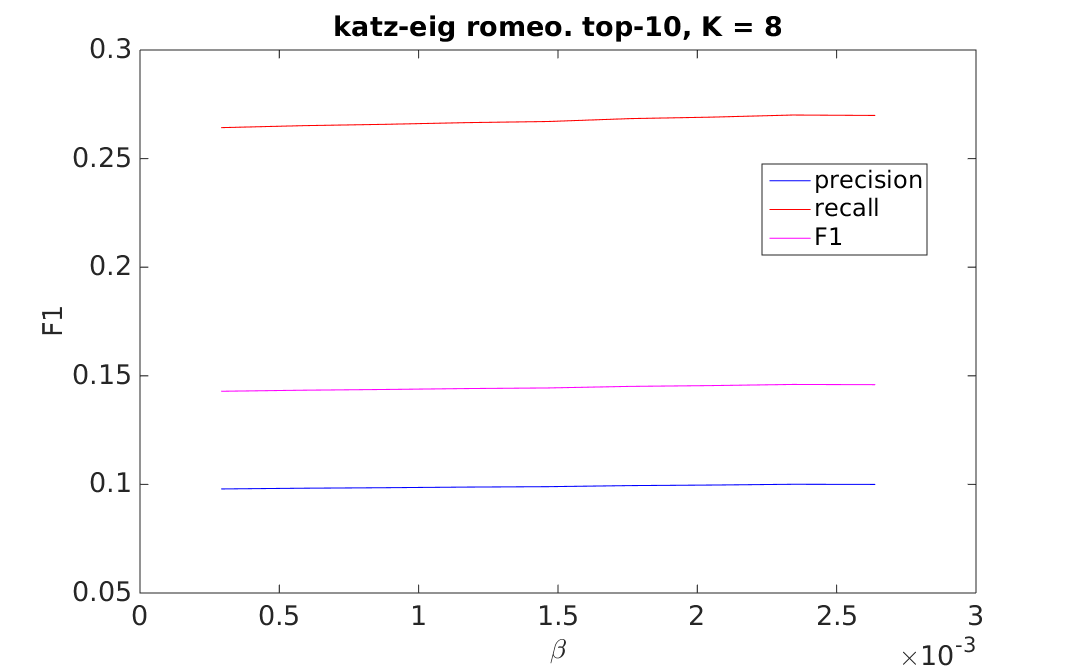
\includegraphics[width=\linewidth]{fig/katzeig_beta/romeo_katzeig_beta.png}
    \captionof{figure}{\textit{movielens1m}.
        $\beta_{max}$ is not the best value with a $2.09\%$ diff between the minimum and the maximum \textit{F1} value.}
\end{minipage}
\end{figure}

\FloatBarrier

The difference between the optimal $\beta$ and an arbitrary selected $\beta$ isn't very large. Even smaller is the difference between the optimal $\beta$ and $\beta_{max}$.  \Tableref{tab:katzeig_beta} is a summary of the evaluated values.

\begin{table}[h!]
    \centering
    \begin{tabular}{| c | r | r | r | r | l |}
        \hline
        \textbf{dataset}        & \textbf{diff between $\beta_{opt}$ and $\beta_{max}$ }    & \textbf{diff between $f_{min}$ and $f_{max}$} \\ \hline

        \textit{alphaS}         & 0~\%      & 2.0~\%    \\ \hline
        \textit{eswc2015books}  & 0~\%      & 0\%       \\ \hline
        \textit{eswc2015movies} & 0.039~\%  & 0.28~\%   \\ \hline
        \textit{movielens1m}    & 0.41~\%   & 0.41~\%   \\ \hline
        \textit{romeo}          & 0.072~\%  & 2.1~\%    \\ \hline


    \end{tabular}
    \caption{A summary of evaluating different $\beta$. $\beta_{max} = \frac{1}{\|A_{train}\|_2}$ is the maximally examined $\beta$ and $\beta_{opt}$ is the optimal $\beta$ found in the range $0 < \beta \leq \beta_{max}$. $K$ is individually optimized for the different datasets. $f_{min}$ and $f_{max}$ are the minimal and maximal \textit{F1} values obtained.}
    \label{tab:katzeig_beta}
\end{table}

\FloatBarrier

\newpage


The $K$-rank approximation represents different available models for \textit{katz-eig}. The following plots show different values of $K$, evaluated w.r.t. the test set. $\beta = \frac{1}{\|A_{train}\|}_2$ for all datasets. $K_{m}$ is the value of $K$ which gives the best \textit{F-measure} for each dataset.

\FloatBarrier

\begin{figure}[h!]
\centering
\begin{minipage}{.5\textwidth}
    \centering
    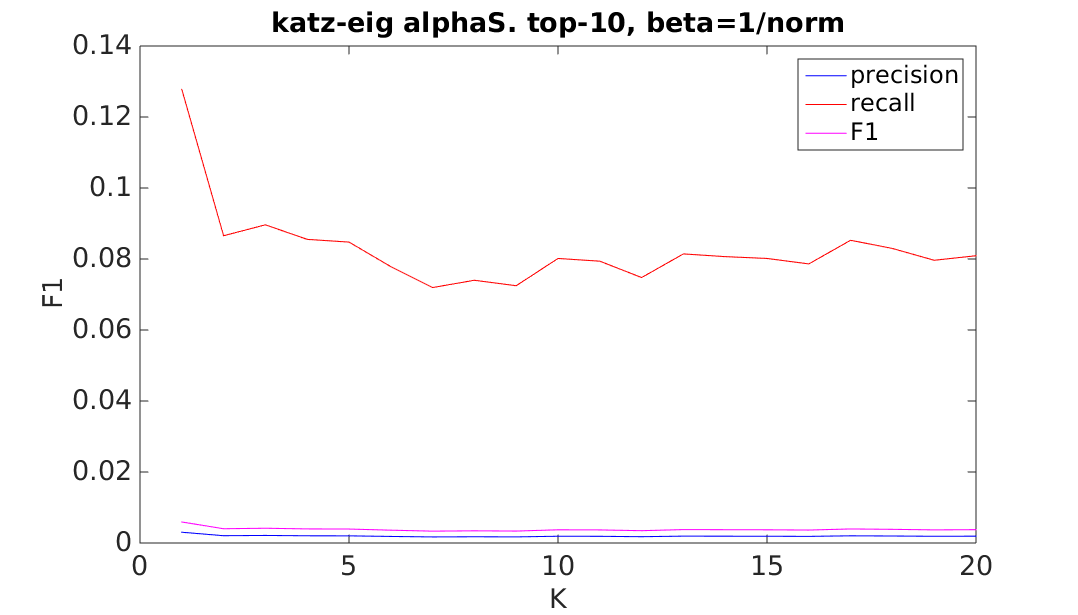
\includegraphics[width=\linewidth]{fig/katzeig_k/alphaS_katzeig_K.png}
    \captionof{figure}{\textit{alphaS} $K_{m} = 13$}
\end{minipage}%
\begin{minipage}{.5\textwidth}
    \centering
    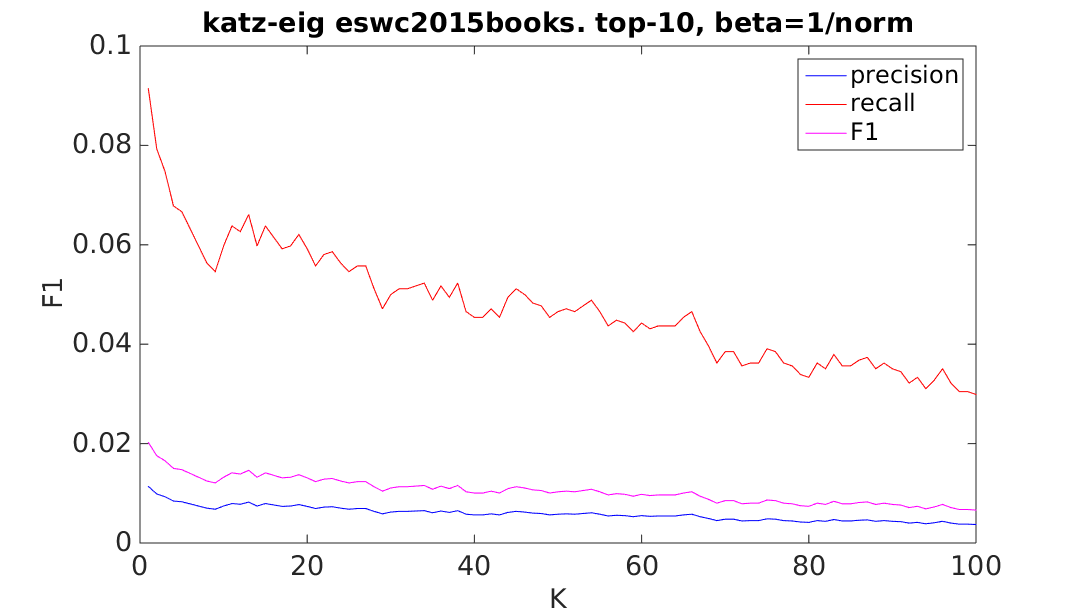
\includegraphics[width=\linewidth]{fig/katzeig_k/eswc2015books_katzeig_K.png}
    \captionof{figure}{\textit{eswc2015books} $K_{m} = 1$}
\end{minipage}
\end{figure}

\begin{figure}[h!]
\centering
\begin{minipage}{.5\textwidth}
    \centering
    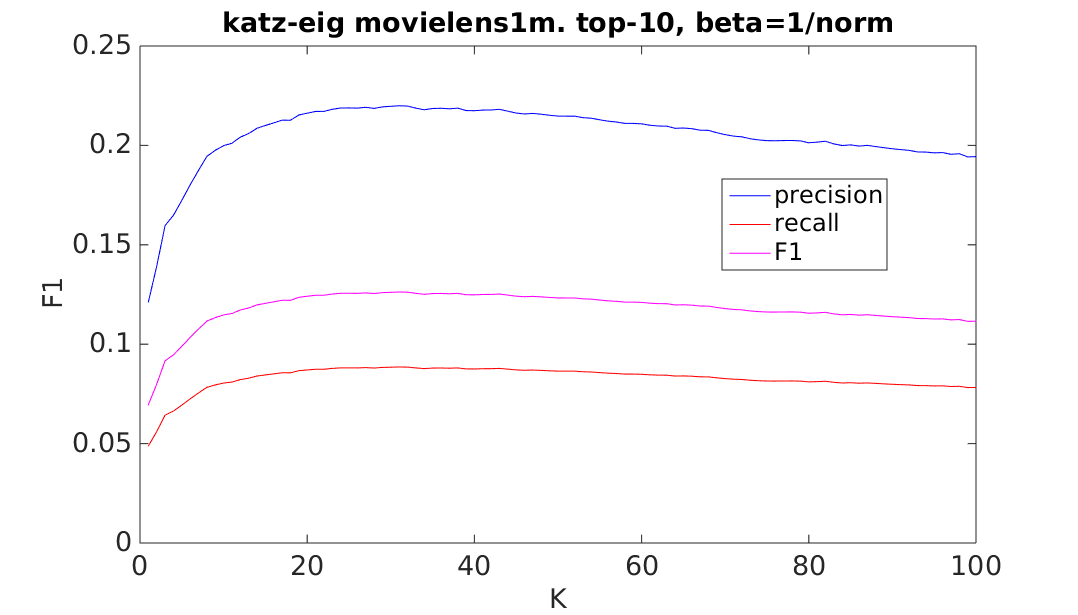
\includegraphics[width=\linewidth]{fig/katzeig_k/movielens_katzeig_K.png}
    \captionof{figure}{\textit{movielens1m} $K_{m} = 31$}
\end{minipage}%
\begin{minipage}{.5\textwidth}
    \centering
    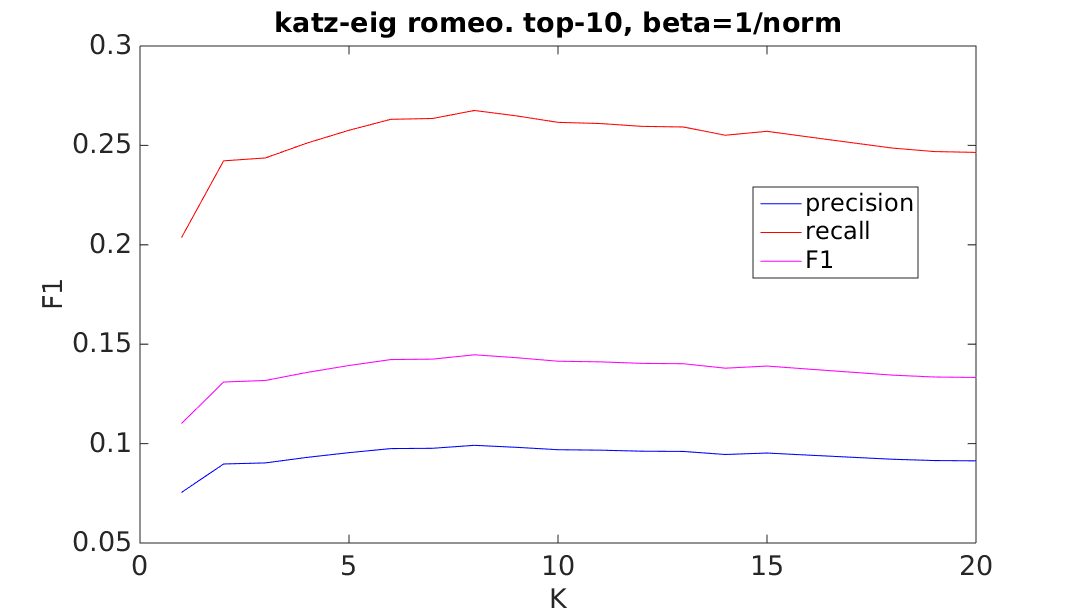
\includegraphics[width=\linewidth]{fig/katzeig_k/romeo_katzeig_K.png}
    \captionof{figure}{\textit{romeo} $K_{m} = 8$}
\end{minipage}
\end{figure}

\Warning[TODO]{ Plot of \textit{eswc2015movies}? }

%\begin{figure}[h!]
%\centering
%\begin{minipage}{.5\textwidth}
    %\centering
    %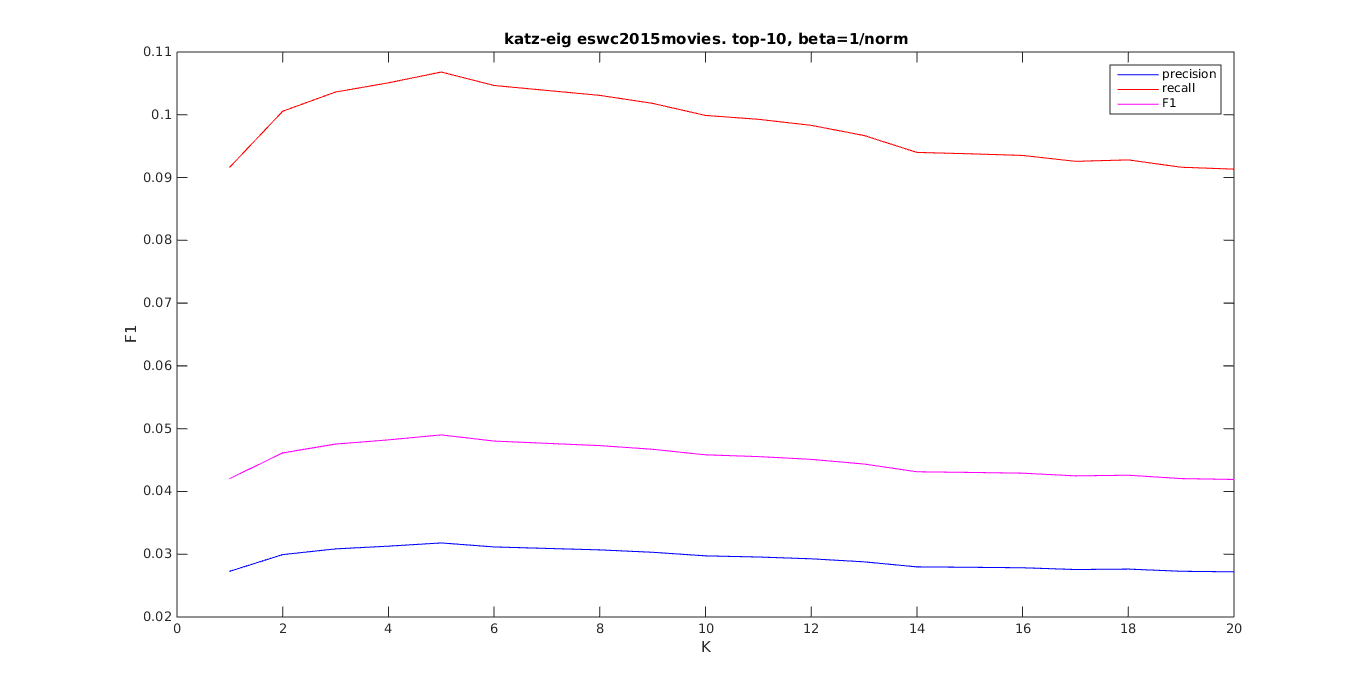
\includegraphics[width=\linewidth]{fig/katzeig_k/eswc2015movies_katzeig_K.png}
    %\captionof{figure}{\textit{eswc2015movies} $K_{m} = 5$}
%\end{minipage}%
%\begin{minipage}{.5\textwidth}
    %\centering
    %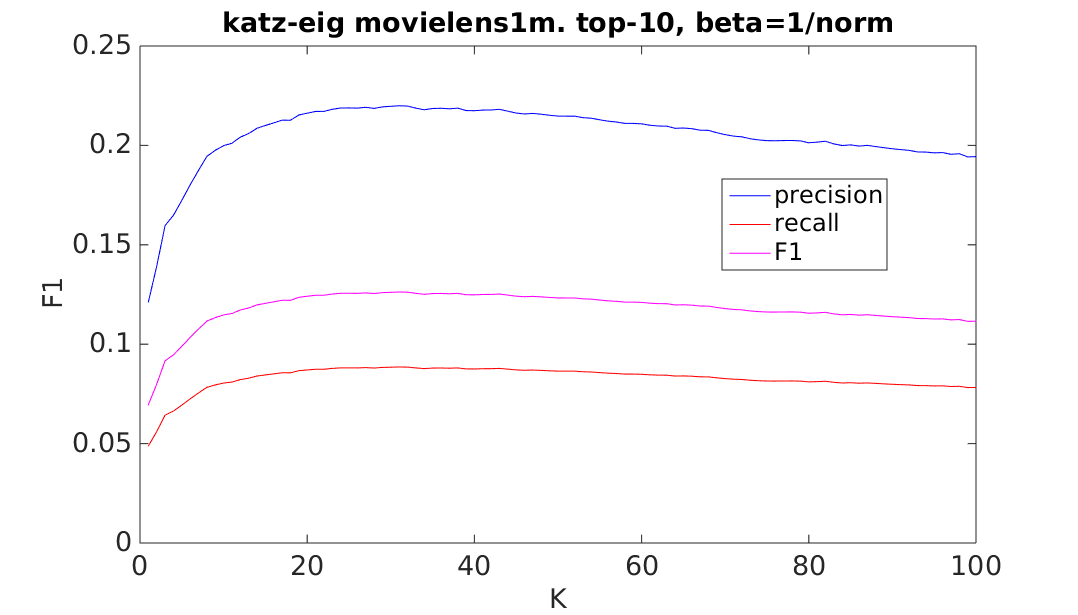
\includegraphics[width=\linewidth]{fig/katzeig_k/movielens_katzeig_K.png}
    %\captionof{figure}{\textit{movielens1m} $K_{m} = 31$}
%\end{minipage}
%\end{figure}

%\begin{figure}[h!]
%%\centering
%\begin{minipage}{.5\textwidth}
    %%\centering
    %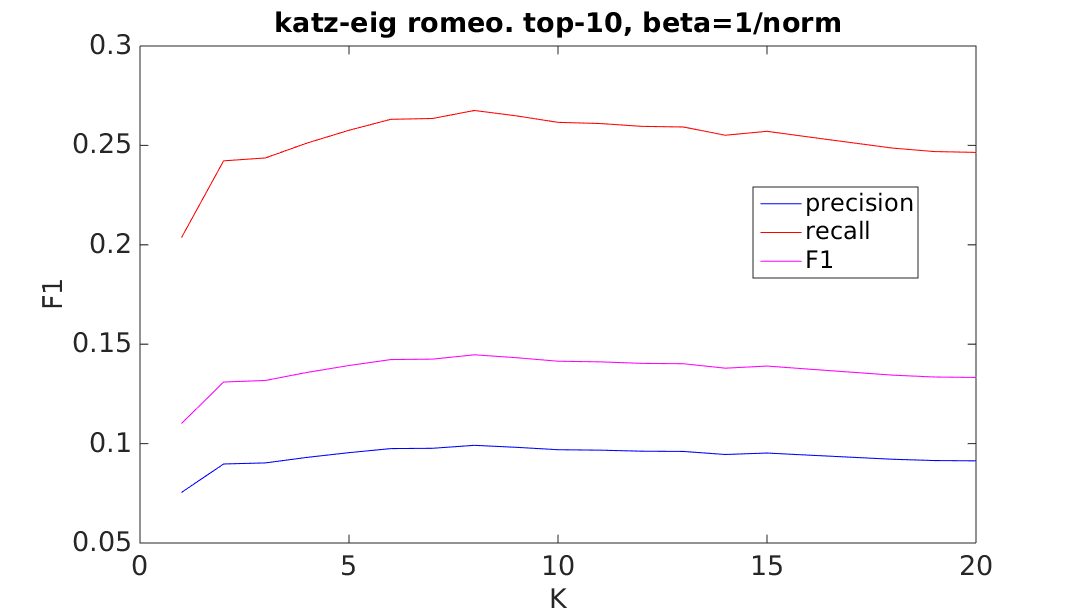
\includegraphics[width=\linewidth]{fig/katzeig_k/romeo_katzeig_K.png}
    %\captionof{figure}{\textit{romeo} $K_{m} = 8$}
%\end{minipage}%
%\end{figure}

\FloatBarrier

The function space w.r.t. $K$ is fairly smooth if not entirely convex. \textit{eswc2015books} is an outlier with a low optimal value $K = 1$ and many local optima. The other datasets display more smooth functions, but there are clear local optima with both \textit{alphaS} and \textit{romeo}.

Also of note is that the functions start to decline at different $K$. \textit{eswc2015movies} declines already at $K = 5$ but it's only at around $K = 30$ \textit{movielens1m} starts to decline. As noted earlier \textit{eswc2015books} has it's optima already at $K = 1$.



\section{Evaluation}\label{sec:method:eval}

Recommendation quality was evaluated using \textit{Precision}, \textit{Recall} and \textit{F-measure} with top-10 recommendations. Focus was on \textit{F-measure} as a combined measure of \textit{Precision} and \textit{Recall}.

The following steps describes the steps taken to produce evaluations given the training, validation and test sets $A_{train}$, $A_{val}$ and $A_{test}$:

\begin{enumerate}
    \item Produce recommendation predictions $p_{u, i}$ from $A_{train}$ with the chosen algorithm.
    \item Transform $p_{u, i}$ to a set of binary recommendations $r_{u, i}$ using the top-10 most predicted items for each user, by the process described in \chapterref{cha:theory}.
    \item Evaluate \textit{F-measure}, as described in \sectionref{sec:background:theory:eval}, with $e_{u, i}$ representing $A_{val}$ or $A_{test}$, depending on which set to evaluate against.
\end{enumerate}

If not explicitly noted, the evaluation set was the test set.



\newpage
\section{Random thoughts and things}

Binary classifier, likes?

Things I need to research more:

\begin{enumerate}
    \item Various optimization techniques?
    \item Collaborative filtering, neighbours? \cite{hu2008collaborative}
    \item Matrix factorization.
\end{enumerate}

Things to write about:

\begin{enumerate}
    \item LinkAnalysis. Written about in \cite{huang2007comparison}.
\end{enumerate}


\subsection{\cite{hu2008collaborative}}

Usually minimize a cost function, with regularization such as:

\begin{equation}
    \min_{x_*, y_*} \sum_{r_{u,i} \text{ is known} } (r_{ui} - x_{u}^T y_i)^2 + \lambda(\|x_u\|^2 + \|y_i\|^2)
\end{equation}

Model as:

\begin{equation}
    p_{ui} = \begin{cases}
        1 \quad r_{ui} > 0 \\
        0 \quad r_{ui} = 0
    \end{cases}
\end{equation}

Here $p_{ui}$ describes our confidence level for user $u$ to like item $i$.

$r_{ui}$ described as how fully did user $u$ consume item $i$. For example if the value is $0.7$ then the user watched $70\%$ of the show. This is used by \cite{hu2008collaborative}.

We however just use binary values.

\cite{hu2008collaborative} use this cost function:

\begin{equation}
    \min_{x_*, y_*} \sum_{u,i} c_{ui} (p_{ui} - x_{u}^T y_i)^2 + \lambda(\sum_{u} \|x_u\|^2 + \sum_{i} \|y_i\|^2)
\end{equation}

This function accounts for (1) varying confidence levels (we don't need it as we don't use implicit ones) and (2) should account for all pairs, not just observer (not sure what to think about this).

Use cross-validation to select $\lambda$.

This cost function is very slow to compute though. Can we make do with the original one?

Here $x_{u}^T y_i$ are our predicted values!

Usually we use stochastic gradient descent to find parameters \cite{hu2008collaborative}.

Describes link-analysis here.

\Warning[TODO]{Mention discoveries!}

Using $\eta$, but uses it as a constant. My findings are different. Possibly negative values?

Using $\gamma$ in the range 0 to 1, but larger ones are also good.







\chapter{Related Work}\label{cha:relwork}

%\textit{Need to anchor problem formulation here!}

\textit{Practically complete until halftime eval!}

A lot of research has been put into recommender systems \citep{bobadilla2013recommender}. Most articles are concerned with improving accuracy of recommender system results, such as optimizing for \rmse. This was the case for the popular Netflix Prize \citep{bennett2007netflix} which was concerned with recommending movies given user ratings for other movies. Explicit feedback recommender systems continue to be a well researched area \citep{bobadilla2013recommender}.

According to \citep{lai2012hybrid} the Top-N Recommendation problem is the real problem of many on-line recommender systems and it's common to seek improvements for recommendation quality, using \textit{Precision} or \textit{Recall} \citep{bobadilla2013recommender}. The 2nd Linked Open Data-enabled Recommender Systems Challenge
\footnote{2nd Linked Open Data-enabled Recommender Systems Challenge, 2015. \url{http://sisinflab.poliba.it/events/lod-recsys-challenge-2015/}}
is another competition which focuses on improving recommendation quality for the Top-N Recommendation problem as well as additional objectives such as \textit{diversity} \citep{bobadilla2013recommender}.

Implicit feedback systems have grown in popularity and are also being researched \citep{hu2008collaborative, bobadilla2013recommender}. Together with the research many versions of different recommender systems have been implemented, with recommender systems becoming more and more popular \citep{bobadilla2013recommender}. One of the most popular types are hybrid recommender systems which combine different types of data and algorithms \citep{bobadilla2013recommender, lai2012hybrid}. This was the winning approach for the Netflix Prize which combined 107 different algorithms in different ways to produce the final recommendations
\footnote{ Netflix: Recommendations beyond 5 stars (Part 1), 2012. \url{http://techblog.netflix.com/2012/04/netflix-recommendations-beyond-5-stars.html} }.

A related approach is to organize the data into different subsets or clusters and then make recommendations using these subsets. This was negatively evaluated by \citep{cacheda2011comparison} however more positive results were given by a \textit{Clustered Low-Rank Approximation} \citep{niklas, savas2011clustered}.  This was evaluated for user ratings using \rmse and speed benefits were theorized upon but not evaluated.

The \textit{link-analysis} algorithm compared favorably in recommendation quality by \citep{huang2007comparison}. But without any analysis of the algorithm's parameters and no mention of the relative speed of the algorithm.  Similarly \textit{katz-eig} had some positive recommendation quality results \citep{shin2012multi} but no parameter analysis and no mention of the algorithm's speed.

There is research for how to optimize and learn models for other algorithms, but no such research has been done for \textit{link-analysis} or \textit{katz-eig}.

%The link-analysis algorithm is introduced by \citep{huang2004link} and used by \citep{huang2007comparison}. They do not do an in-depth analyze of different values for $\eta$ nor $\gamma$, they only note the best values they found.
%They evaluate the different algorithms using \textit{precision}, \textit{recall}, \textit{F-measure} and \textit{rank score}.
%\Warning[TODO]{ Reformulate }

%The katz-eig algorithm was introduced in \citep{katz1953new}, described by \citep{liben2007link}, used by \citep{shin2012multi}. Some positive results in recommendation quality but no speed evaluation. No mention of parameter optimization.
%\Warning[TODO]{ Read articles, reformulate, remove unnecessary citations }


%\chapter{Theory}\label{cha:theory}


\subsection{Model}\label{sec:background:theory:model}

Given a set of users $U$, a set of items $I$ and an interaction history $h_{u, i}$ given in \textit{unweighted binary form}

\begin{equation}\label{eq:hist}
    h_{u, i} = \begin{cases}
        1 \quad \text{if user $u$ has interacted with item $i$} \\
        0 \quad \text{otherwise}
    \end{cases}
\end{equation}

the \textit{recommender problem} is defined by producing a set of recommendations $r_{u, i}$

\begin{equation}\label{eq:binrec}
    r_{u, i} = \begin{cases}
        1 \quad \text{if item $i$ is recommended to user $u$} \\
        0 \quad \text{otherwise}
    \end{cases}
\end{equation}

to maximize the probability that user $u$ will want to interact with item $i$ in the future, for all users and items.  When $r_{u, i}$ is binary this is a \textit{binary classification} problem. This definition is applicable for \textit{implicit feedback} systems which passively track different sorts of user behaviour. For example link following, interaction time and purchase history.

The recommender problem can be extended to the \textit{Top-N recommender problem} by introducing constraints \eqref{eq:constrain_N} which states that only $N$ recommendations can be presented for each user.

\begin{equation}\label{eq:constrain_N}
    \sum_i r_{u, i} \leq N \quad \forall u
\end{equation}


A variation of the recommender problem is when the interaction history is in \textit{weighted form}, when the values increase with each interaction

\begin{equation}\label{eq:whist}
    h_{u, i} = \begin{cases}
        x \quad \text{user $u$ has interacted $x$ times with item $i$} \\
        0 \quad \text{otherwise}
    \end{cases}
\end{equation}

for example $h_{u, i} = 2$ means that the user $u$ has interacted with item $i$ 2 times. It is possible to allow \textit{implicit feedback} systems to log partial interactions, so $h_{u, i} = 0.7$ could mean that user $u$ has watched 70\% of the movie $i$, in the context of movie watching. \citep{hu2008collaborative}

The converse of \textit{implicit feedback} is \textit{explicit feedback} where the users give direct input regarding their preferences, for example with movie ratings or with likes and dislikes.  Here the definition of the interaction history $h_{u, i}$ is the users' rating history.

\begin{equation}
    h_{u, i} = \begin{cases}
        x \quad \text{the rating $x$ user $u$ gave item $i$} \\
        \emptyset \quad \text{if the user $u$ did not rate item $i$}
    \end{cases}
\end{equation}

\Warning[TODO]{ Uses h for all equations? }

With ratings $r_{u, i}$ changes to $r_{u, i} = \hat{x}$ where $\hat{x}$ is the rating user $u$ is predicted to give item $i$.

\section{The link-analysis algorithm}\label{sec:linkanalysis}

%\textit{Cleanup, mostly description from article. Reduce information?}

The \textit{link-analysis} algorithm, as presented by \cite{huang2004link} and further discussed in \cite{huang2007comparison}. See the articles for more information and in-depth examples. What follows is a condensed description of how the algorithm works.

The algorithm is an adaptation of HITS \cite{kleinberg1999authoritative} which is a web page ranking algorithm to the recommendation domain. The original algorithm distinguish between \textit{Authoritative} pages which definitely contain high-quality information and \textit{Hub} pages which are comprehensive lists of links to authoritative pages. \citep{huang2007comparison}

The adaptation to the recommendation domain is achieved by introducing the \textit{product representativeness} score $\PR$ and the \textit{consumer representativeness} score $\CR$.

The \textit{product representativeness} score $\PR(i, u)$ can be seen as a measure of the item $i$'s level of interest with respect to user $u$, or in other words $i$'s authority of $u$'s interests in $i$.

The \textit{consumer representativeness} score $\CR(u, \hat{u})$ measures how well $u$ as a hub for $\hat{u}$ associates with products of interests to $\hat{u}$.

If $h_{u, i}$ is the user-item interaction history as defined by \ref{eq:hist} and $h$ is the interaction matrix then a recursive definition of the authority and hub scores can be defined as

\begin{equation}
    \PR = h' * \CR
\end{equation}

\begin{equation}
    \CR = B * \PR + \CR_0
\end{equation}

Where $B$ is a matrix such that:

\begin{equation}
    B_{u, i} = \frac{ h_{u, i} }{ \left(\sum_{i} h_{u, i}\right)^\gamma }
\end{equation}

Meaning $B$ normalizes the representativeness score a costumer receives from linked products by dividing it with the total number of products the customer is linked to.  $\gamma$ controls the extent to which a consumer is penalized for making many purchases.

$\CR_0$ is defined as

\begin{equation}
    \CR_{i, j}^0 = \begin{cases}
        \eta \quad \text{if } \; i = j \\
        0    \quad \text{otherwise}
    \end{cases}
\end{equation}

in other words $\CR_0 = \eta * I_M$ where $I_M$ is an $M x M$ identity matrix and $M$ is the number of users.  It is included to maintain the high representativeness score for the target users themselves. This also necessitates a normalization step to keep the values on a consistent level.

In summary the \textit{link-analysis} algorithm follow these steps:

\begin{enumerate}
    \item Construct the interaction matrix $A$ and the associating matrix $B$.

    \item Set $\CR_0 = \eta * I_M$.
    \item At each iteration $t = 1, \ldots, t_{max}$ perform:

        \begin{enumerate}
            \item $\PR_t = h' * \CR_{t- 1}$
            \item $\CR_t = B * \PR_t$
            \item Normalize $\CR_t$ so each column adds up to 1
            \item $\CR_t = \CR_t + \CR_0$
        \end{enumerate}

        Repeat until convergence.

    \item Predicted user-item interaction is given by $\mathit{pval} = \PR'$.

\end{enumerate}

There are two parameters to the algorithm: $\gamma$ and $\eta$.
%\Warning[TODO]{ Describe them, what's their purpose }



\subsection{katz-eig}

There are two parameters to \textit{katz-eig}: $\beta$, the link diminishing factor and $K$ specifying the $K$-rank approximation. $\beta$ is a continous value satisfying $0 < \beta \leq \frac{1}{\|A_{train}\|_2}$. If $\beta = 0$ then the algorithm will only output 0 and if $\beta > \frac{1}{\|A_{train}\|_2}$ the iterations will not converge. $K > 0$ is a discrete value.

What follows is plots over both of the parameters $K$ and $\beta$. The plots are evaluated using \textit{F-measure} w.r.t. the test set using top-10 recommendations.

\begin{figure}[h!]
\centering
\begin{minipage}{.5\textwidth}
    \centering
    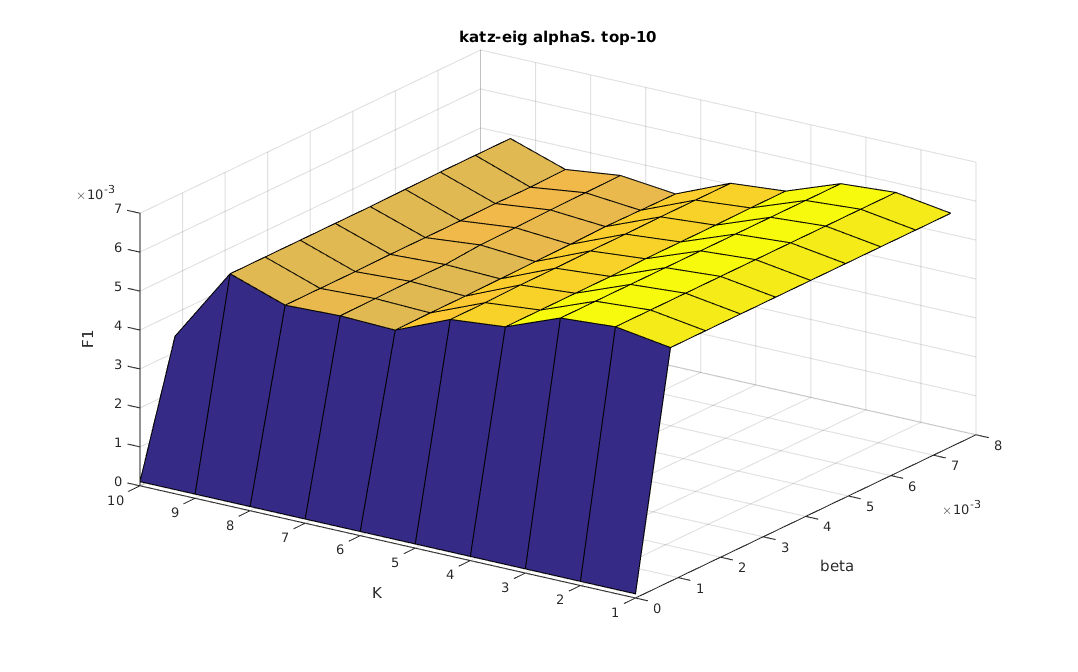
\includegraphics[width=\linewidth]{fig/katzeig_beta_k/alphaS_katzeig.png}
    \captionof{figure}{\textit{alphaS}}
\end{minipage}%
\begin{minipage}{.5\textwidth}
    \centering
    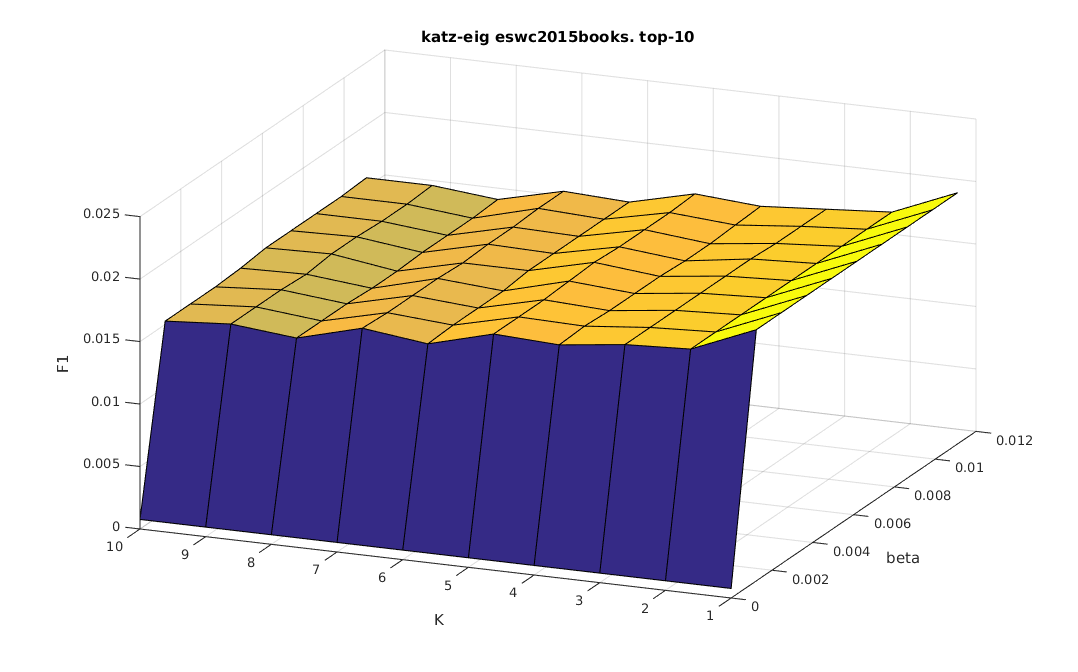
\includegraphics[width=\linewidth]{fig/katzeig_beta_k/eswc2015books_katzeig.png}
    \captionof{figure}{\textit{eswc2015books}}
\end{minipage}
\end{figure}

\begin{figure}[h!]
\centering
\begin{minipage}{.5\textwidth}
    \centering
    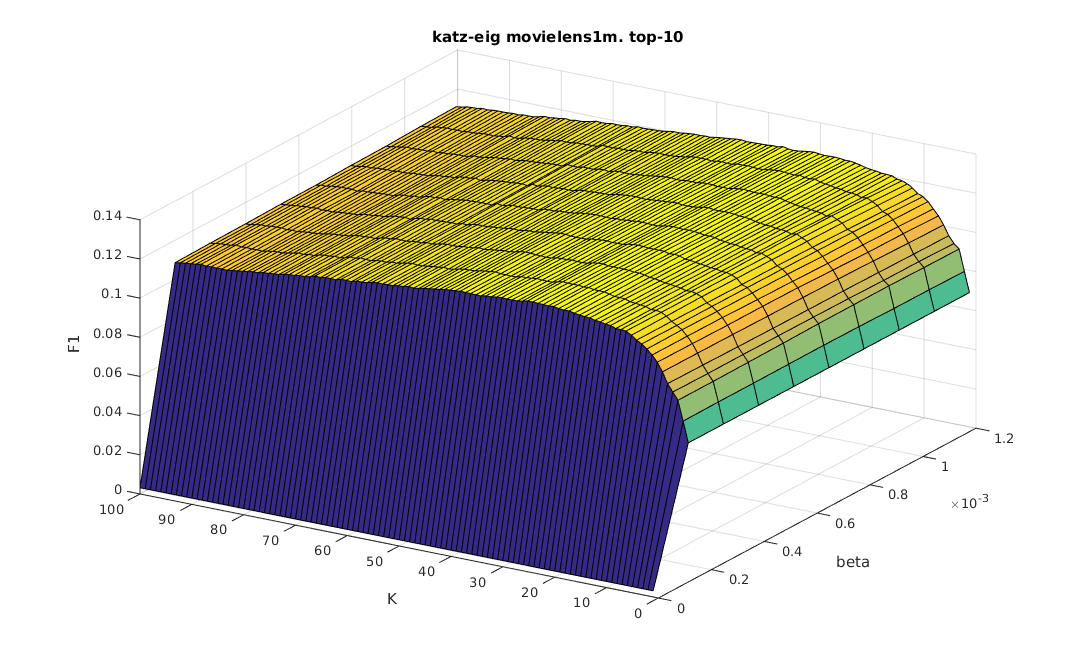
\includegraphics[width=\linewidth]{fig/katzeig_beta_k/movielens_katzeig.png}
    \captionof{figure}{\textit{movielens1m}}
\end{minipage}%
\begin{minipage}{.5\textwidth}
    \centering
    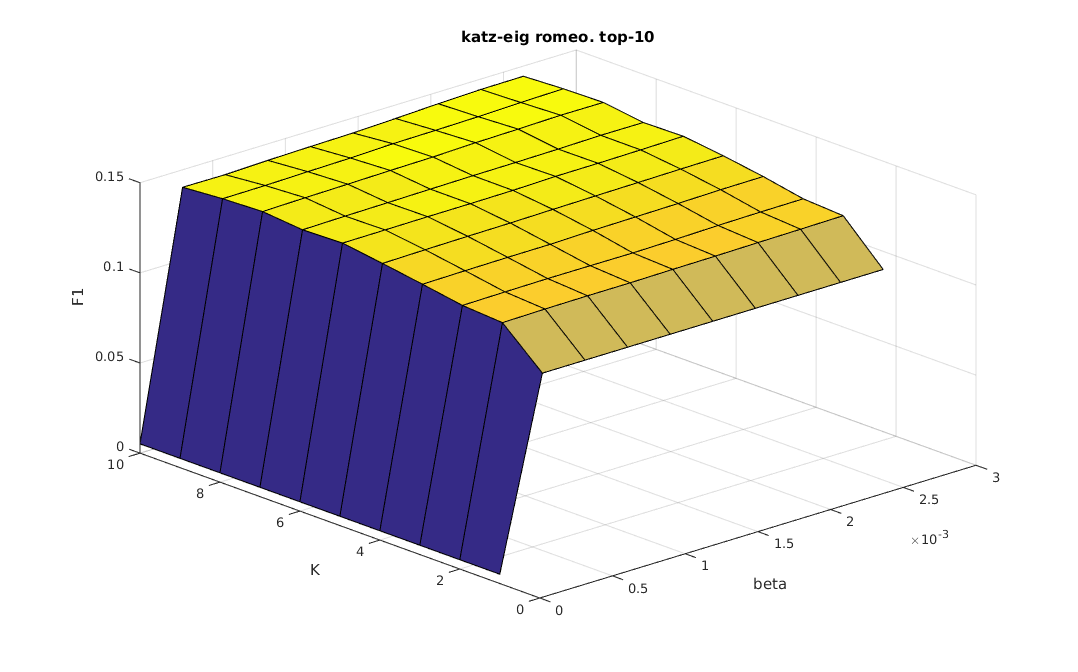
\includegraphics[width=\linewidth]{fig/katzeig_beta_k/romeo_katzeig.png}
    \captionof{figure}{\textit{romeo}}
\end{minipage}
\end{figure}




It seems like $beta$ doesn't have a very big impact on the function value. Some plots with a fixed $K$ follows to better see differences.

The range examined is $0 < \beta \leq \beta_{max} = \frac{1}{\|A_{train}\|_2}$ with a $K$ selected to fit the specific dataset. Again evaluated using \textit{Precision}, \textit{Recall} and \textit{F-measure} w.r.t. the test set using the top-10 recommendations.

\FloatBarrier

\begin{figure}[h!]
\centering
\begin{minipage}{.5\textwidth}
    \centering
    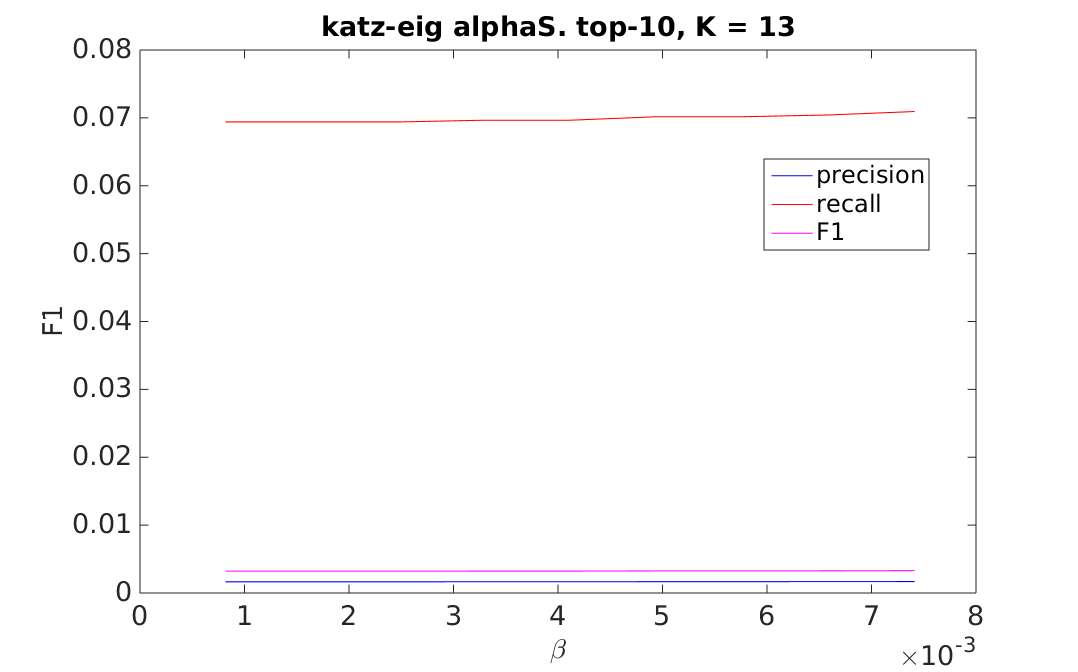
\includegraphics[width=\linewidth]{fig/katzeig_beta/alphaS_katzeig_beta.png}
    \captionof{figure}{\textit{alphaS}.
        $\beta_{max}$ is the best value with a $1.9\%$ diff between the minimum and the maximum \textit{F1} value.}
\end{minipage}%
\begin{minipage}{.5\textwidth}
    \centering
    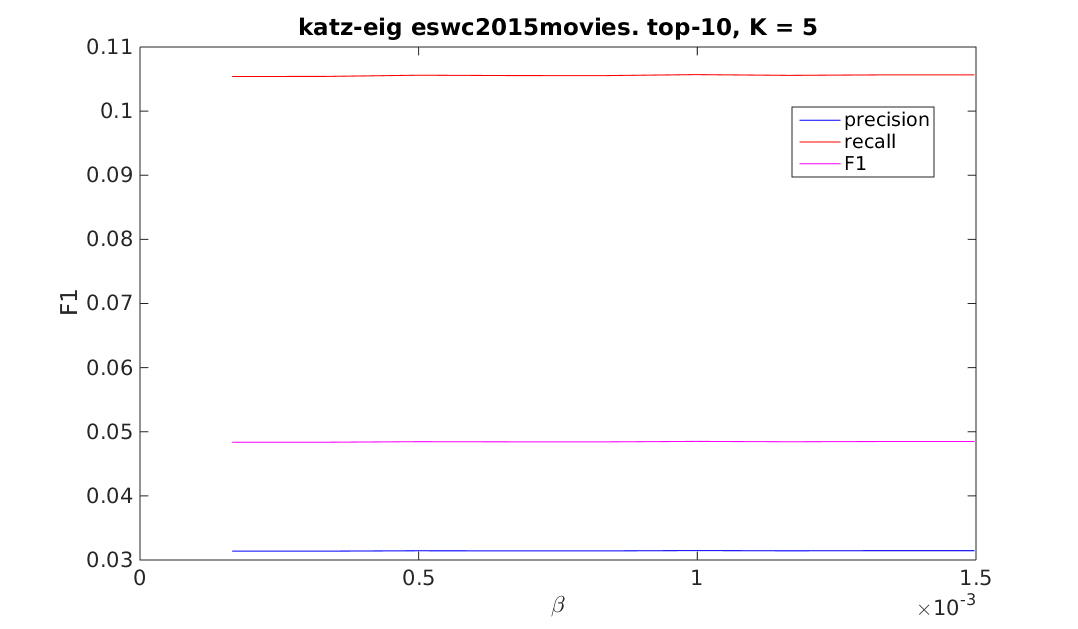
\includegraphics[width=\linewidth]{fig/katzeig_beta/eswc2015movies_katzeig_beta.png}
    \captionof{figure}{\textit{eswc2015movies}.
        $\beta_{max}$ is not the best value with a $0.3\%$ diff between the minimum and the maximum \textit{F1} value.}
\end{minipage}
\end{figure}

\begin{figure}[h!]
\centering
\begin{minipage}{.5\textwidth}
    \centering
    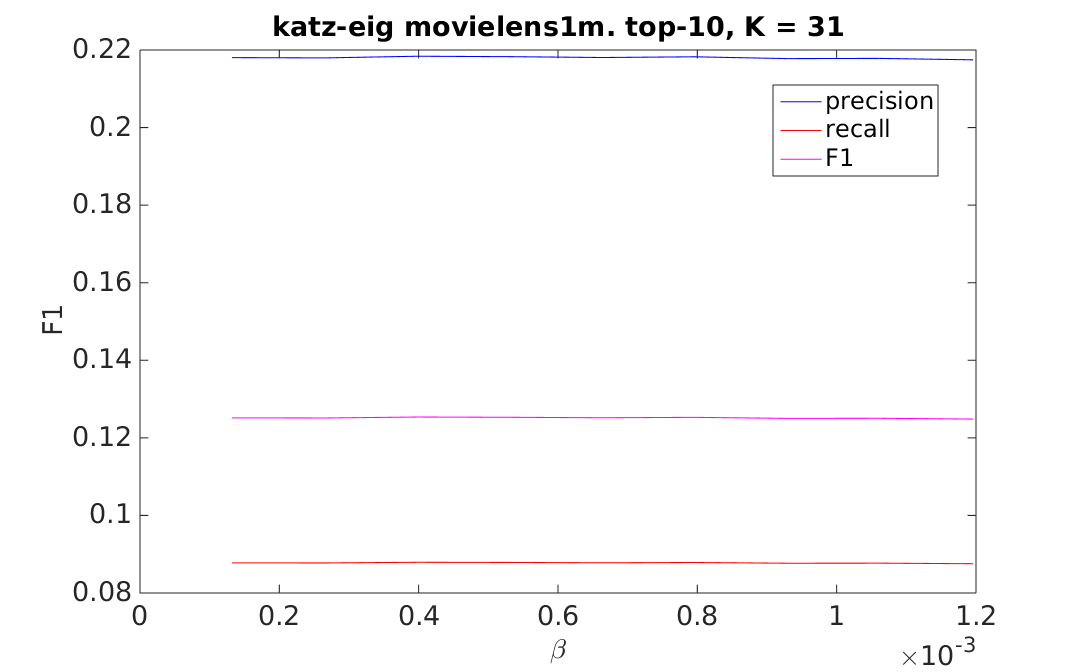
\includegraphics[width=\linewidth]{fig/katzeig_beta/movielens_katzeig_beta.png}
    \captionof{figure}{\textit{movielens1m}.
        $\beta_{max}$ is not the best value with a $0.41\%$ diff between the minimum and the maximum \textit{F1} value.}
\end{minipage}%
\begin{minipage}{.5\textwidth}
    \centering
    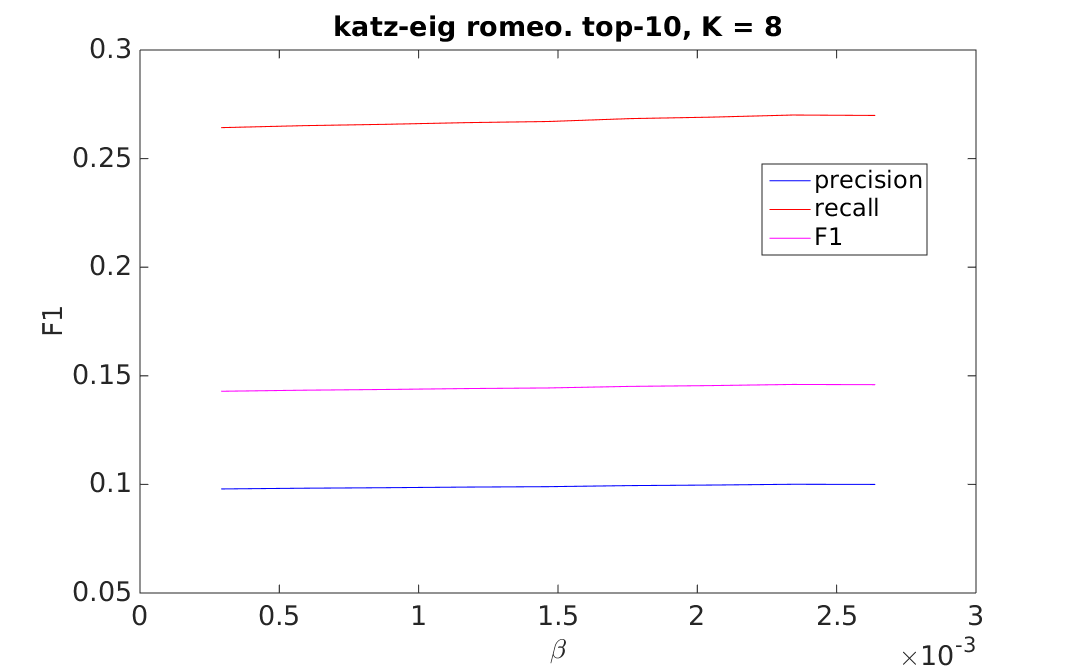
\includegraphics[width=\linewidth]{fig/katzeig_beta/romeo_katzeig_beta.png}
    \captionof{figure}{\textit{movielens1m}.
        $\beta_{max}$ is not the best value with a $2.09\%$ diff between the minimum and the maximum \textit{F1} value.}
\end{minipage}
\end{figure}

\FloatBarrier

The difference between the optimal $\beta$ and an arbitrary selected $\beta$ isn't very large. Even smaller is the difference between the optimal $\beta$ and $\beta_{max}$.  \Tableref{tab:katzeig_beta} is a summary of the evaluated values.

\begin{table}[h!]
    \centering
    \begin{tabular}{| c | r | r | r | r | l |}
        \hline
        \textbf{dataset}        & \textbf{diff between $\beta_{opt}$ and $\beta_{max}$ }    & \textbf{diff between $f_{min}$ and $f_{max}$} \\ \hline

        \textit{alphaS}         & 0~\%      & 2.0~\%    \\ \hline
        \textit{eswc2015books}  & 0~\%      & 0\%       \\ \hline
        \textit{eswc2015movies} & 0.039~\%  & 0.28~\%   \\ \hline
        \textit{movielens1m}    & 0.41~\%   & 0.41~\%   \\ \hline
        \textit{romeo}          & 0.072~\%  & 2.1~\%    \\ \hline


    \end{tabular}
    \caption{A summary of evaluating different $\beta$. $\beta_{max} = \frac{1}{\|A_{train}\|_2}$ is the maximally examined $\beta$ and $\beta_{opt}$ is the optimal $\beta$ found in the range $0 < \beta \leq \beta_{max}$. $K$ is individually optimized for the different datasets. $f_{min}$ and $f_{max}$ are the minimal and maximal \textit{F1} values obtained.}
    \label{tab:katzeig_beta}
\end{table}

\FloatBarrier

\newpage


The $K$-rank approximation represents different available models for \textit{katz-eig}. The following plots show different values of $K$, evaluated w.r.t. the test set. $\beta = \frac{1}{\|A_{train}\|}_2$ for all datasets. $K_{m}$ is the value of $K$ which gives the best \textit{F-measure} for each dataset.

\FloatBarrier

\begin{figure}[h!]
\centering
\begin{minipage}{.5\textwidth}
    \centering
    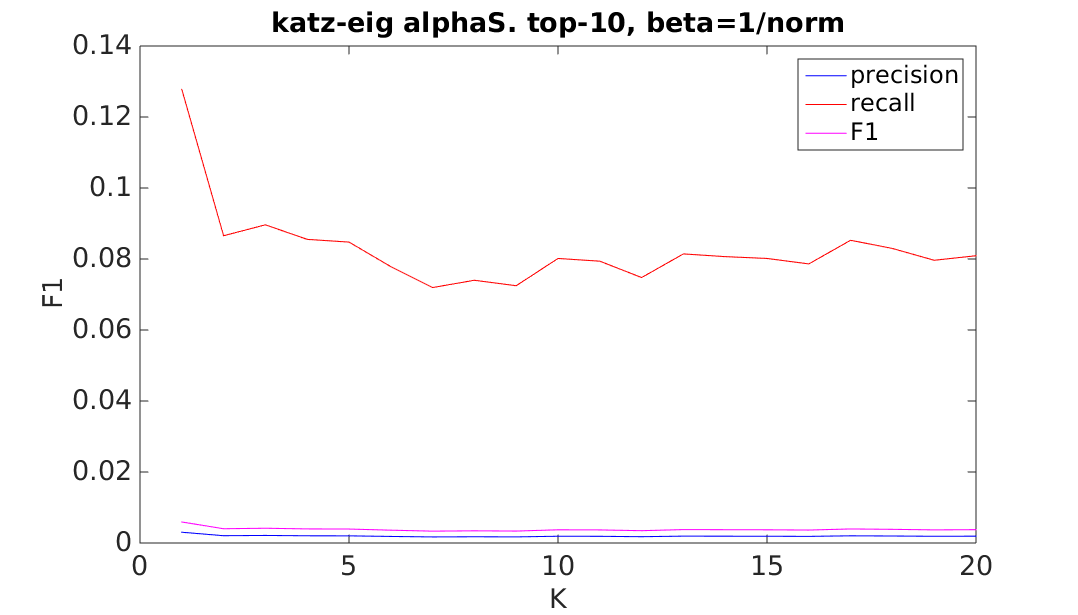
\includegraphics[width=\linewidth]{fig/katzeig_k/alphaS_katzeig_K.png}
    \captionof{figure}{\textit{alphaS} $K_{m} = 13$}
\end{minipage}%
\begin{minipage}{.5\textwidth}
    \centering
    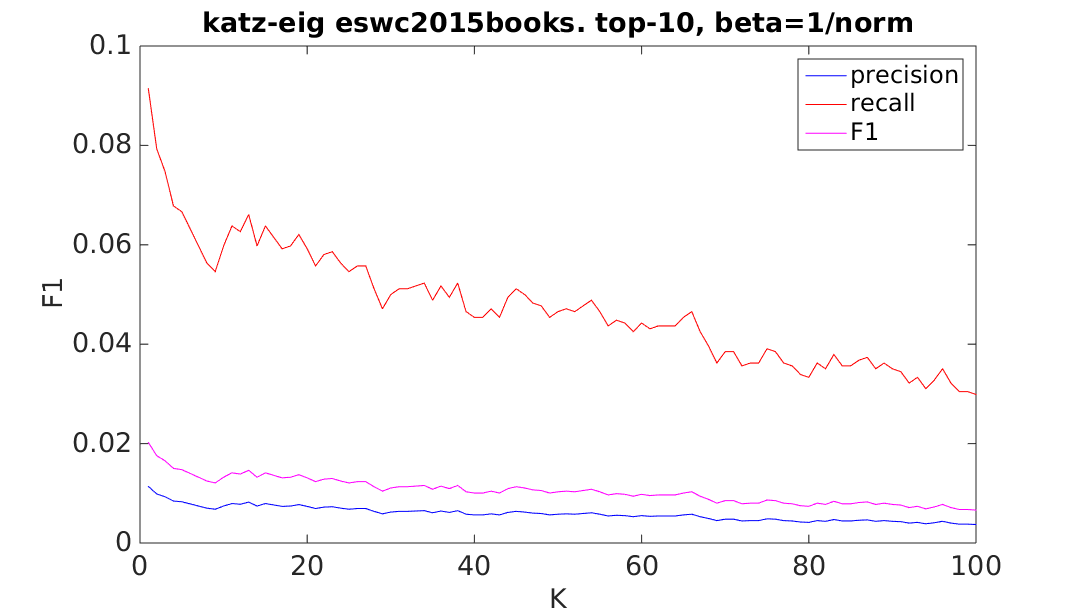
\includegraphics[width=\linewidth]{fig/katzeig_k/eswc2015books_katzeig_K.png}
    \captionof{figure}{\textit{eswc2015books} $K_{m} = 1$}
\end{minipage}
\end{figure}

\begin{figure}[h!]
\centering
\begin{minipage}{.5\textwidth}
    \centering
    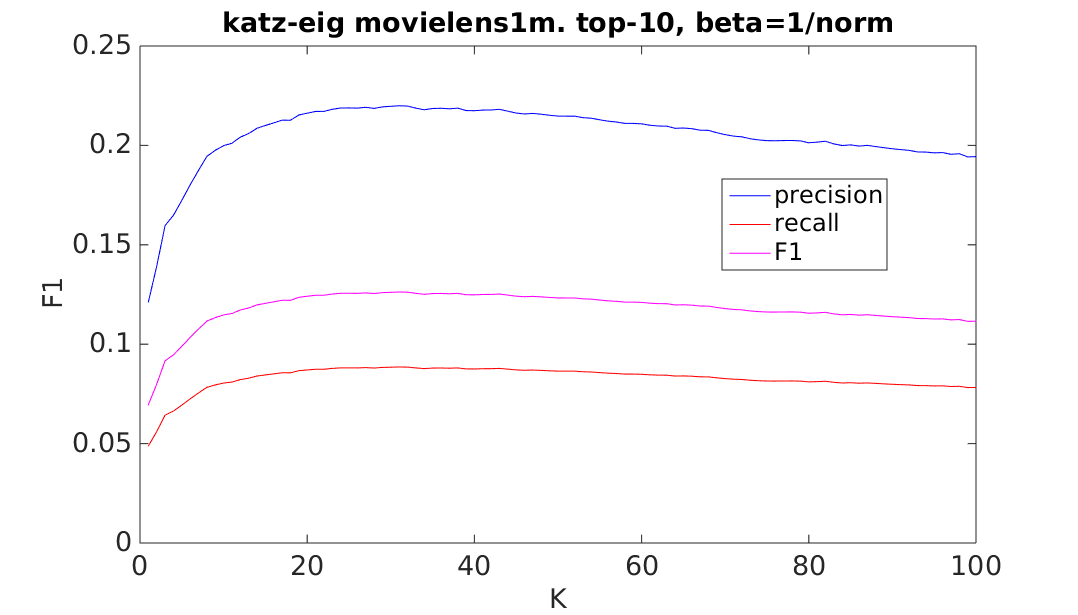
\includegraphics[width=\linewidth]{fig/katzeig_k/movielens_katzeig_K.png}
    \captionof{figure}{\textit{movielens1m} $K_{m} = 31$}
\end{minipage}%
\begin{minipage}{.5\textwidth}
    \centering
    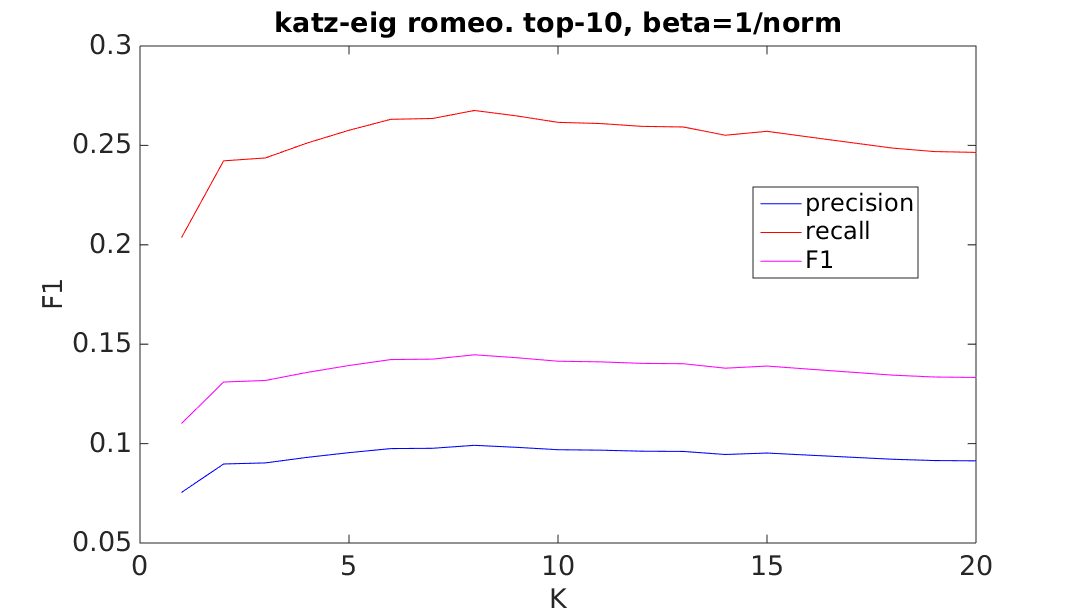
\includegraphics[width=\linewidth]{fig/katzeig_k/romeo_katzeig_K.png}
    \captionof{figure}{\textit{romeo} $K_{m} = 8$}
\end{minipage}
\end{figure}

\Warning[TODO]{ Plot of \textit{eswc2015movies}? }

%\begin{figure}[h!]
%\centering
%\begin{minipage}{.5\textwidth}
    %\centering
    %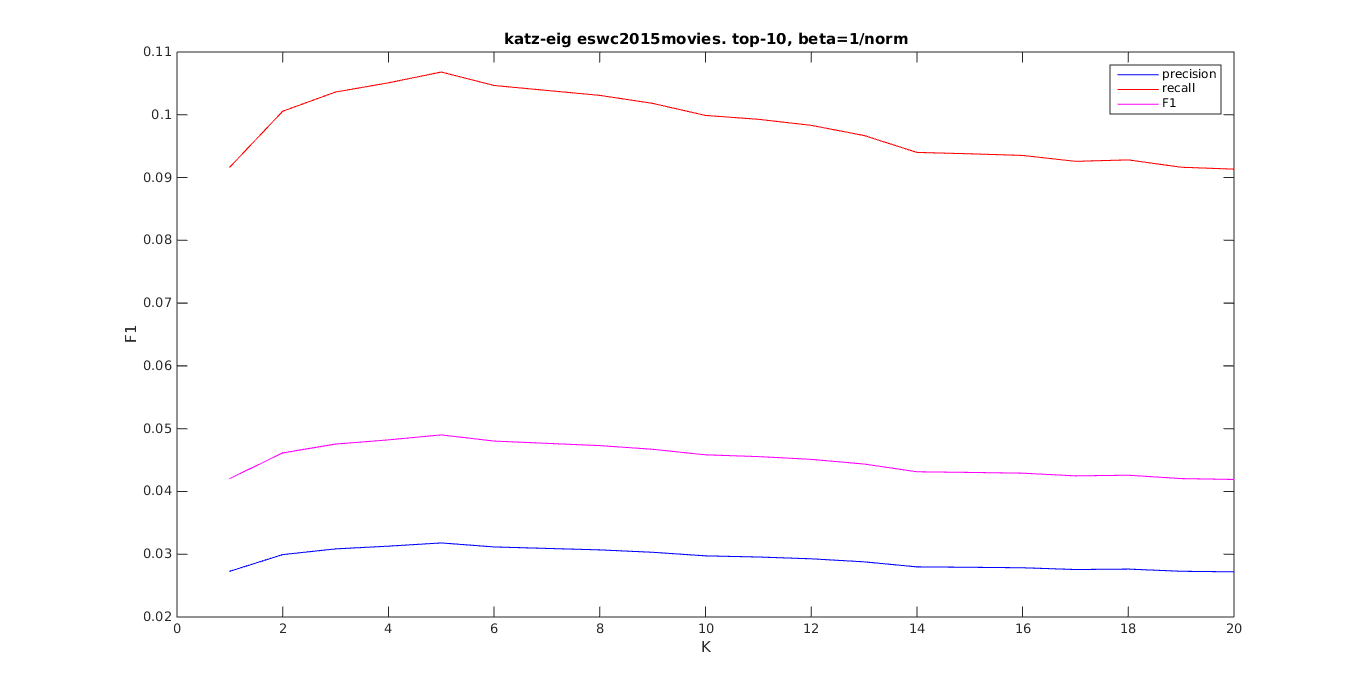
\includegraphics[width=\linewidth]{fig/katzeig_k/eswc2015movies_katzeig_K.png}
    %\captionof{figure}{\textit{eswc2015movies} $K_{m} = 5$}
%\end{minipage}%
%\begin{minipage}{.5\textwidth}
    %\centering
    %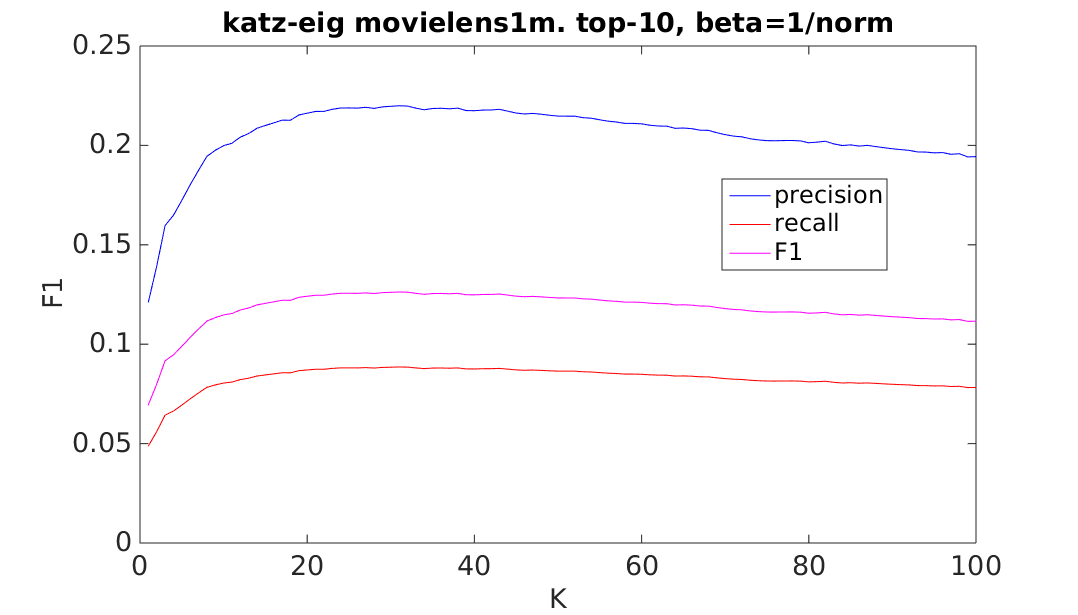
\includegraphics[width=\linewidth]{fig/katzeig_k/movielens_katzeig_K.png}
    %\captionof{figure}{\textit{movielens1m} $K_{m} = 31$}
%\end{minipage}
%\end{figure}

%\begin{figure}[h!]
%%\centering
%\begin{minipage}{.5\textwidth}
    %%\centering
    %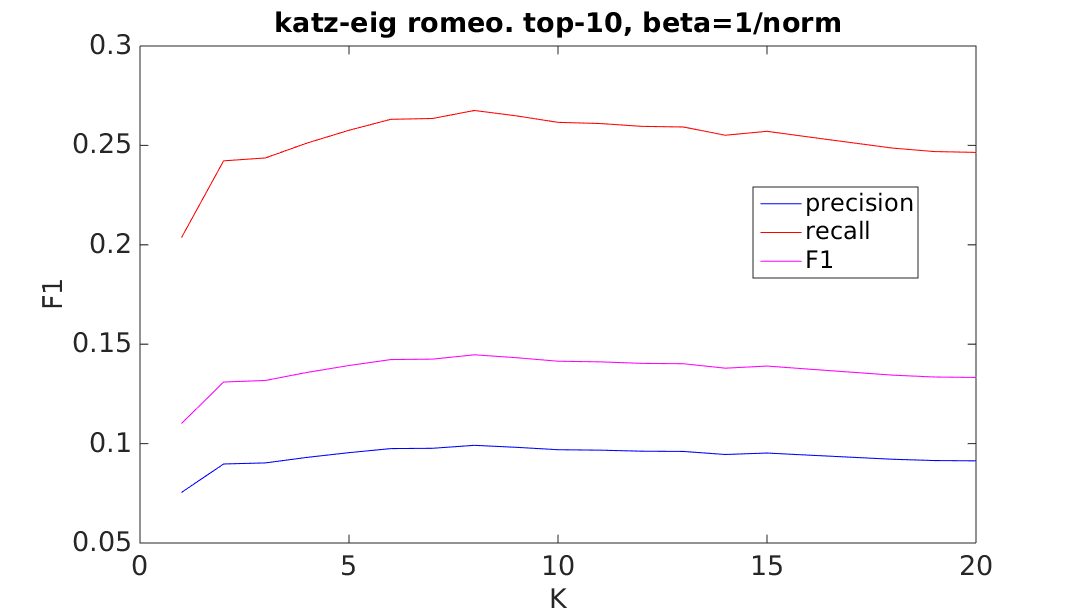
\includegraphics[width=\linewidth]{fig/katzeig_k/romeo_katzeig_K.png}
    %\captionof{figure}{\textit{romeo} $K_{m} = 8$}
%\end{minipage}%
%\end{figure}

\FloatBarrier

The function space w.r.t. $K$ is fairly smooth if not entirely convex. \textit{eswc2015books} is an outlier with a low optimal value $K = 1$ and many local optima. The other datasets display more smooth functions, but there are clear local optima with both \textit{alphaS} and \textit{romeo}.

Also of note is that the functions start to decline at different $K$. \textit{eswc2015movies} declines already at $K = 5$ but it's only at around $K = 30$ \textit{movielens1m} starts to decline. As noted earlier \textit{eswc2015books} has it's optima already at $K = 1$.



\section{Evaluation}\label{sec:method:eval}

Recommendation quality was evaluated using \textit{Precision}, \textit{Recall} and \textit{F-measure} with top-10 recommendations. Focus was on \textit{F-measure} as a combined measure of \textit{Precision} and \textit{Recall}.

The following steps describes the steps taken to produce evaluations given the training, validation and test sets $A_{train}$, $A_{val}$ and $A_{test}$:

\begin{enumerate}
    \item Produce recommendation predictions $p_{u, i}$ from $A_{train}$ with the chosen algorithm.
    \item Transform $p_{u, i}$ to a set of binary recommendations $r_{u, i}$ using the top-10 most predicted items for each user, by the process described in \chapterref{cha:theory}.
    \item Evaluate \textit{F-measure}, as described in \sectionref{sec:background:theory:eval}, with $e_{u, i}$ representing $A_{val}$ or $A_{test}$, depending on which set to evaluate against.
\end{enumerate}

If not explicitly noted, the evaluation set was the test set.



\newpage
\section{Random thoughts and things}

Binary classifier, likes?

Things I need to research more:

\begin{enumerate}
    \item Various optimization techniques?
    \item Collaborative filtering, neighbours? \cite{hu2008collaborative}
    \item Matrix factorization.
\end{enumerate}

Things to write about:

\begin{enumerate}
    \item LinkAnalysis. Written about in \cite{huang2007comparison}.
\end{enumerate}


\subsection{\cite{hu2008collaborative}}

Usually minimize a cost function, with regularization such as:

\begin{equation}
    \min_{x_*, y_*} \sum_{r_{u,i} \text{ is known} } (r_{ui} - x_{u}^T y_i)^2 + \lambda(\|x_u\|^2 + \|y_i\|^2)
\end{equation}

Model as:

\begin{equation}
    p_{ui} = \begin{cases}
        1 \quad r_{ui} > 0 \\
        0 \quad r_{ui} = 0
    \end{cases}
\end{equation}

Here $p_{ui}$ describes our confidence level for user $u$ to like item $i$.

$r_{ui}$ described as how fully did user $u$ consume item $i$. For example if the value is $0.7$ then the user watched $70\%$ of the show. This is used by \cite{hu2008collaborative}.

We however just use binary values.

\cite{hu2008collaborative} use this cost function:

\begin{equation}
    \min_{x_*, y_*} \sum_{u,i} c_{ui} (p_{ui} - x_{u}^T y_i)^2 + \lambda(\sum_{u} \|x_u\|^2 + \sum_{i} \|y_i\|^2)
\end{equation}

This function accounts for (1) varying confidence levels (we don't need it as we don't use implicit ones) and (2) should account for all pairs, not just observer (not sure what to think about this).

Use cross-validation to select $\lambda$.

This cost function is very slow to compute though. Can we make do with the original one?

Here $x_{u}^T y_i$ are our predicted values!

Usually we use stochastic gradient descent to find parameters \cite{hu2008collaborative}.

Describes link-analysis here.

\Warning[TODO]{Mention discoveries!}

Using $\eta$, but uses it as a constant. My findings are different. Possibly negative values?

Using $\gamma$ in the range 0 to 1, but larger ones are also good.







\section{Methodology}\label{sec:disc:method}

\textit{Discuss and critique for the methods chosen.}

\textit{Also discuss sources.}

The usage of the \textit{movielens1m} dataset can be questioned as the dataset is made up by ratings and then converted to unweighted binary form. This introduces a lot of noise and the question is what conclusions can be drawn from such a dataset.

The evaluation metric of \textit{F-measure} can be questioned/discussed...? Why no cost function? Probably would be better (if could be found, but can it?) ?

Optimization technique interesting to try is bayesian optimization! (can we try it?)

Clustering would be nice to explore (if we don't do it in the thesis).



\section{Results}\label{sec:disc:results}

\textit{How does the results hold up? Compare to theory breakthrough. Anything unusual or surprising?}

\subsection{link-analysis}

Referenced article introduces $\eta$, but treats it as a constant. My findings are different and shows better results for other values, possibly even for negative values.

Similarly $\gamma$ is said to be in the range 0 to 1, but I found that larger ones are good and often even better.


\chapter{Discussion}\label{cha:discussion}

\textit{Can free form sections here}


\section{Results}\label{sec:disc:results}

\textit{How does the results hold up? Compare to theory breakthrough. Anything unusual or surprising?}

\subsection{link-analysis}

Referenced article introduces $\eta$, but treats it as a constant. My findings are different and shows better results for other values, possibly even for negative values.

Similarly $\gamma$ is said to be in the range 0 to 1, but I found that larger ones are good and often even better.




\section{Methodology}\label{sec:disc:method}

\textit{Discuss and critique for the methods chosen.}

\textit{Also discuss sources.}

The usage of the \textit{movielens1m} dataset can be questioned as the dataset is made up by ratings and then converted to unweighted binary form. This introduces a lot of noise and the question is what conclusions can be drawn from such a dataset.

The evaluation metric of \textit{F-measure} can be questioned/discussed...? Why no cost function? Probably would be better (if could be found, but can it?) ?

Optimization technique interesting to try is bayesian optimization! (can we try it?)

Clustering would be nice to explore (if we don't do it in the thesis).





\chapter{Conclusions}\label{cha:conclusions}


\section{Results}\label{sec:conclusions:results}


\section{Methodology}\label{sec:conclusions:method}


\section{Bigger picture}\label{sec:conclusions:big}


\Warning[TODO]{Remove Bigger picture??}


\part*{Appendix}
\appendix
\chapter{Nomenclature}\label{cha:nomenclature}

recommendations

e-commerce

true positivies

false positives

false negatives

Precision

Recall

F-measure

ratings

interaction history

interaction count

machine learning

clustering

implicit feedback

explicit feedback


\chapter{Optimized parameters}\label{app:opt_params}

During the thesis values of the algorithms' parmaters which would yield good results are used. This section is a summary of optimized values used to get good values of \textit{F-measure} on the corresponding dataset.

\begin{table}[h!]
    \centering
    \begin{tabular}{| c | c | c | c | c | c | c |}
        \hline
        \textbf{}   & \textit{alphaS}   & \textit{eswc2015books} & \textit{eswc2015movies} & \textit{eswc2015music} & \textit{movielens1m}   & \textit{romeo} \\ \hline
        $K$         & 13                & 1                      & 5                       & 4                       & 31                     & 8              \\ \hline
    \end{tabular}
    \caption{Optimized parameters for \textit{katz-eig}. Found using grid search in $K \leq 100$.}
    \label{tab:katzeig_params_used}
\end{table}

\begin{table}[h!]
    \centering
    \begin{tabular}{| c | c | c | c | c | c | }
        \hline
        \textbf{}   & \textit{alphaS}   & \textit{eswc2015books} & \textit{eswc2015movies} & \textit{movielens1m}   & \textit{romeo} \\ \hline
        $\gamma$    & 1                 & 0                      &                         & 1                      & 2              \\ \hline
        $\eta$      & 4                 & 2.5                    &                         & -3                     & -5             \\ \hline
    \end{tabular}
    \caption{Optimized parameters for \textit{link-analysis}. Found using grid search over $-10 \leq \gamma \leq 10$ and $-10 \leq \eta \leq 10$ with a step size of 1 (or 0.5 as with \textit{eswc2015books}.}
    \label{tab:linkanalysis_params_used}
\end{table}
\Warning[TODO]{ How were they found? }

\Warning[TODO]{ Cleanup this one }



\chapter{SVD}\label{cha:svd}

\textit{svd and svd-k description here}
\Warning[TODO]{ Write! }



\chapter{k-means clustering}\label{app:kmeans}

\textit{k-means clustering explanation here}
\Warning[TODO]{ Write! }


\chapter{Code}\label{app:code}


\section{ESWC reader plugin}\label{sec:eswc_plugin}

\lstinputlisting[language=python]{src/eswc.py}



\chapter{Random thoughts}

\textit{Remove later, collect random things.}


\section{Theory}

\section{Related Work}

A common deficiency for evaluation metrics is the lack of formalization. The metrics themselves are well defined but implementation details differ and are sometimes missing which can lead to different results between similar experiments.
\Warning[TODO]{ Move to evaluation chapter? }
\Warning[TODO]{ Comment on strange evaluation results using precision/recall/F1 definitions from another article? }


Both algorithms are nearest neighbour algorithms? Also collaborative filtering? Or?

They are model based algorithms though.

Ignore the cold start problem.

Ignore explaining recommendations.

Different evaluation strategies include: Novelty Precision/Recall. Coverage. Trust Recall.

See \citep{bobadilla2013recommender} for definitions.

\begin{enumerate}
    \item prediction evaluations (accuracy) (Quality of the predictions)

        Such as Mean Absolute Error (MAE), Root of Mean Square Error (RMSE), Normalized Mean Average Error (NMAE)

    \item evaluations for recommendations as sets (precision) (Quality of set of recommendations)

        Precision, Recall, Receiver Operating Characteristic (ROC)

    \item evaluation as ranked lists (Quality of list of recommendations)

        half-life, discounted cumulative gain

    \item diversity metrics
\end{enumerate}

Cross validation techniques:
    random sub-sampling and k-fold cross validation

ESWC 2014 discussions by \citep{di2014linked}, \citep{heitmann2014semstim}, \citep{ostuni2014linked}. Read them!




\backmatter

% XXX commented out for final thesis!
%\nocite{*}
\bibliography{myrefs}

\printindex

\end{document}
